\documentclass[12pt,a4paper]{article}
\usepackage[utf8]{inputenc}
\usepackage[czech]{babel}
\usepackage{datetime, graphicx, float}
\usepackage[colorlinks=true,linkcolor=blue,urlcolor=green]{hyperref}
\renewcommand{\dateseparator}{. }
\begin{document}

\title{Simulované ochlazování: Problém batohu}
\author{Dominik Plíšek}
\date{\dmyyyydate\today}
\maketitle

\tableofcontents

\section*{Úvod}

Jakožto pokročilou iterativní metodu pro řešení problému batohu (a následně SAT) jsem zvolil simulované ochlazování. Tato metoda začíná na určité teplotě, kterou postupně snižuje. Teplota určuje, jak moc je pravděpodobné, že metoda rozhodne přestoupit v jedné iteraci do stavu, který má horší hodnotu optimalizačního kritéria než stav aktuální. Zpočátku je tedy silnější diversifikace, postupně přibývá intensifikace, čili konvergence k určitému (lokálnímu) minimu optimalizační funkce.

Všechny experimenty jsem prováděl na první čtyřiceti předmětné instanci ze souboru instancí z Eduxu, která má tento formát:

9550 40 600 14 223 38 230 3 54 1 214 13 118 4 147 15 16 2 104 5 56 49 154 40 106 24 234 18 34 33 195 7 74 10 129 12 159 42 37 41 10 11 185 6 243 45 87 32 57 20 87 9 26 16 201 39 0 23 128 39 194 21 10 46 1 8 28 30 59 26 130 35 160 22 91 34 180 19 16 31 1 17 72

Dle metody dynamického programování má tato instance jako optimální řešení cenu 4068.

\section{Omezující podmínka}

Problém batohu má z hlediska simulovaného ochlazování tu vlastnost, že obsahuje omezující podmínku kapacity, která přímo brání vylepšování optimalizačního kritéria. Je možné, že náhodně vybraný sousední stav není řešením, protože přesahuje kapacitu batohu. Tento problém je možné řešit různě, například způsobem zakomponování penalizace za přeskok na nepoužitelné řešení, která je pak zaúčtována v optimalizačním kritériu.

Já jsem se rozhodl implementovat takový postup, že dojde-li ke skoku na stav nevyhovující omezující podmínce, vrátím se zpět a vybírám nového souseda, aniž bych tento skok započítal do celkového počtu skoků při zjišťování zmrznutí (viz sekce \ref{freeze}) nebo do celkového počtu skoků k horšímu v případě zjišťování počáteční teploty (viz sekce \ref{startingTemp}).

\section{Varianty}

Jedním z rozhodnutí, které je třeba učinit, je způsob získání počáteční teploty. Tu lze volit fixně. Pak se ale může stát, že ji zvolíme příliš vysoko a metoda bude neefektivní, protože se bude dlouho potácet, aniž by konvergovala k nějakému minimu. To je vidět na obrázku \ref{tooHighStart}. Případně jej můžeme zvolit příliš nízko, přičemž pak nastane situace, kdy metoda rychle uvízne v lokálním minimu a vrátí nepříliš optimální výsledek, viz obrázek \ref{tooLowStart}. Oba tyto grafy představují reálné běhy metody nad výše uvedenou instancí při koeficientu ochlazování 0.80 a dynamicky odvozenou spodní hranicí teploty.

\begin{figure}[H]
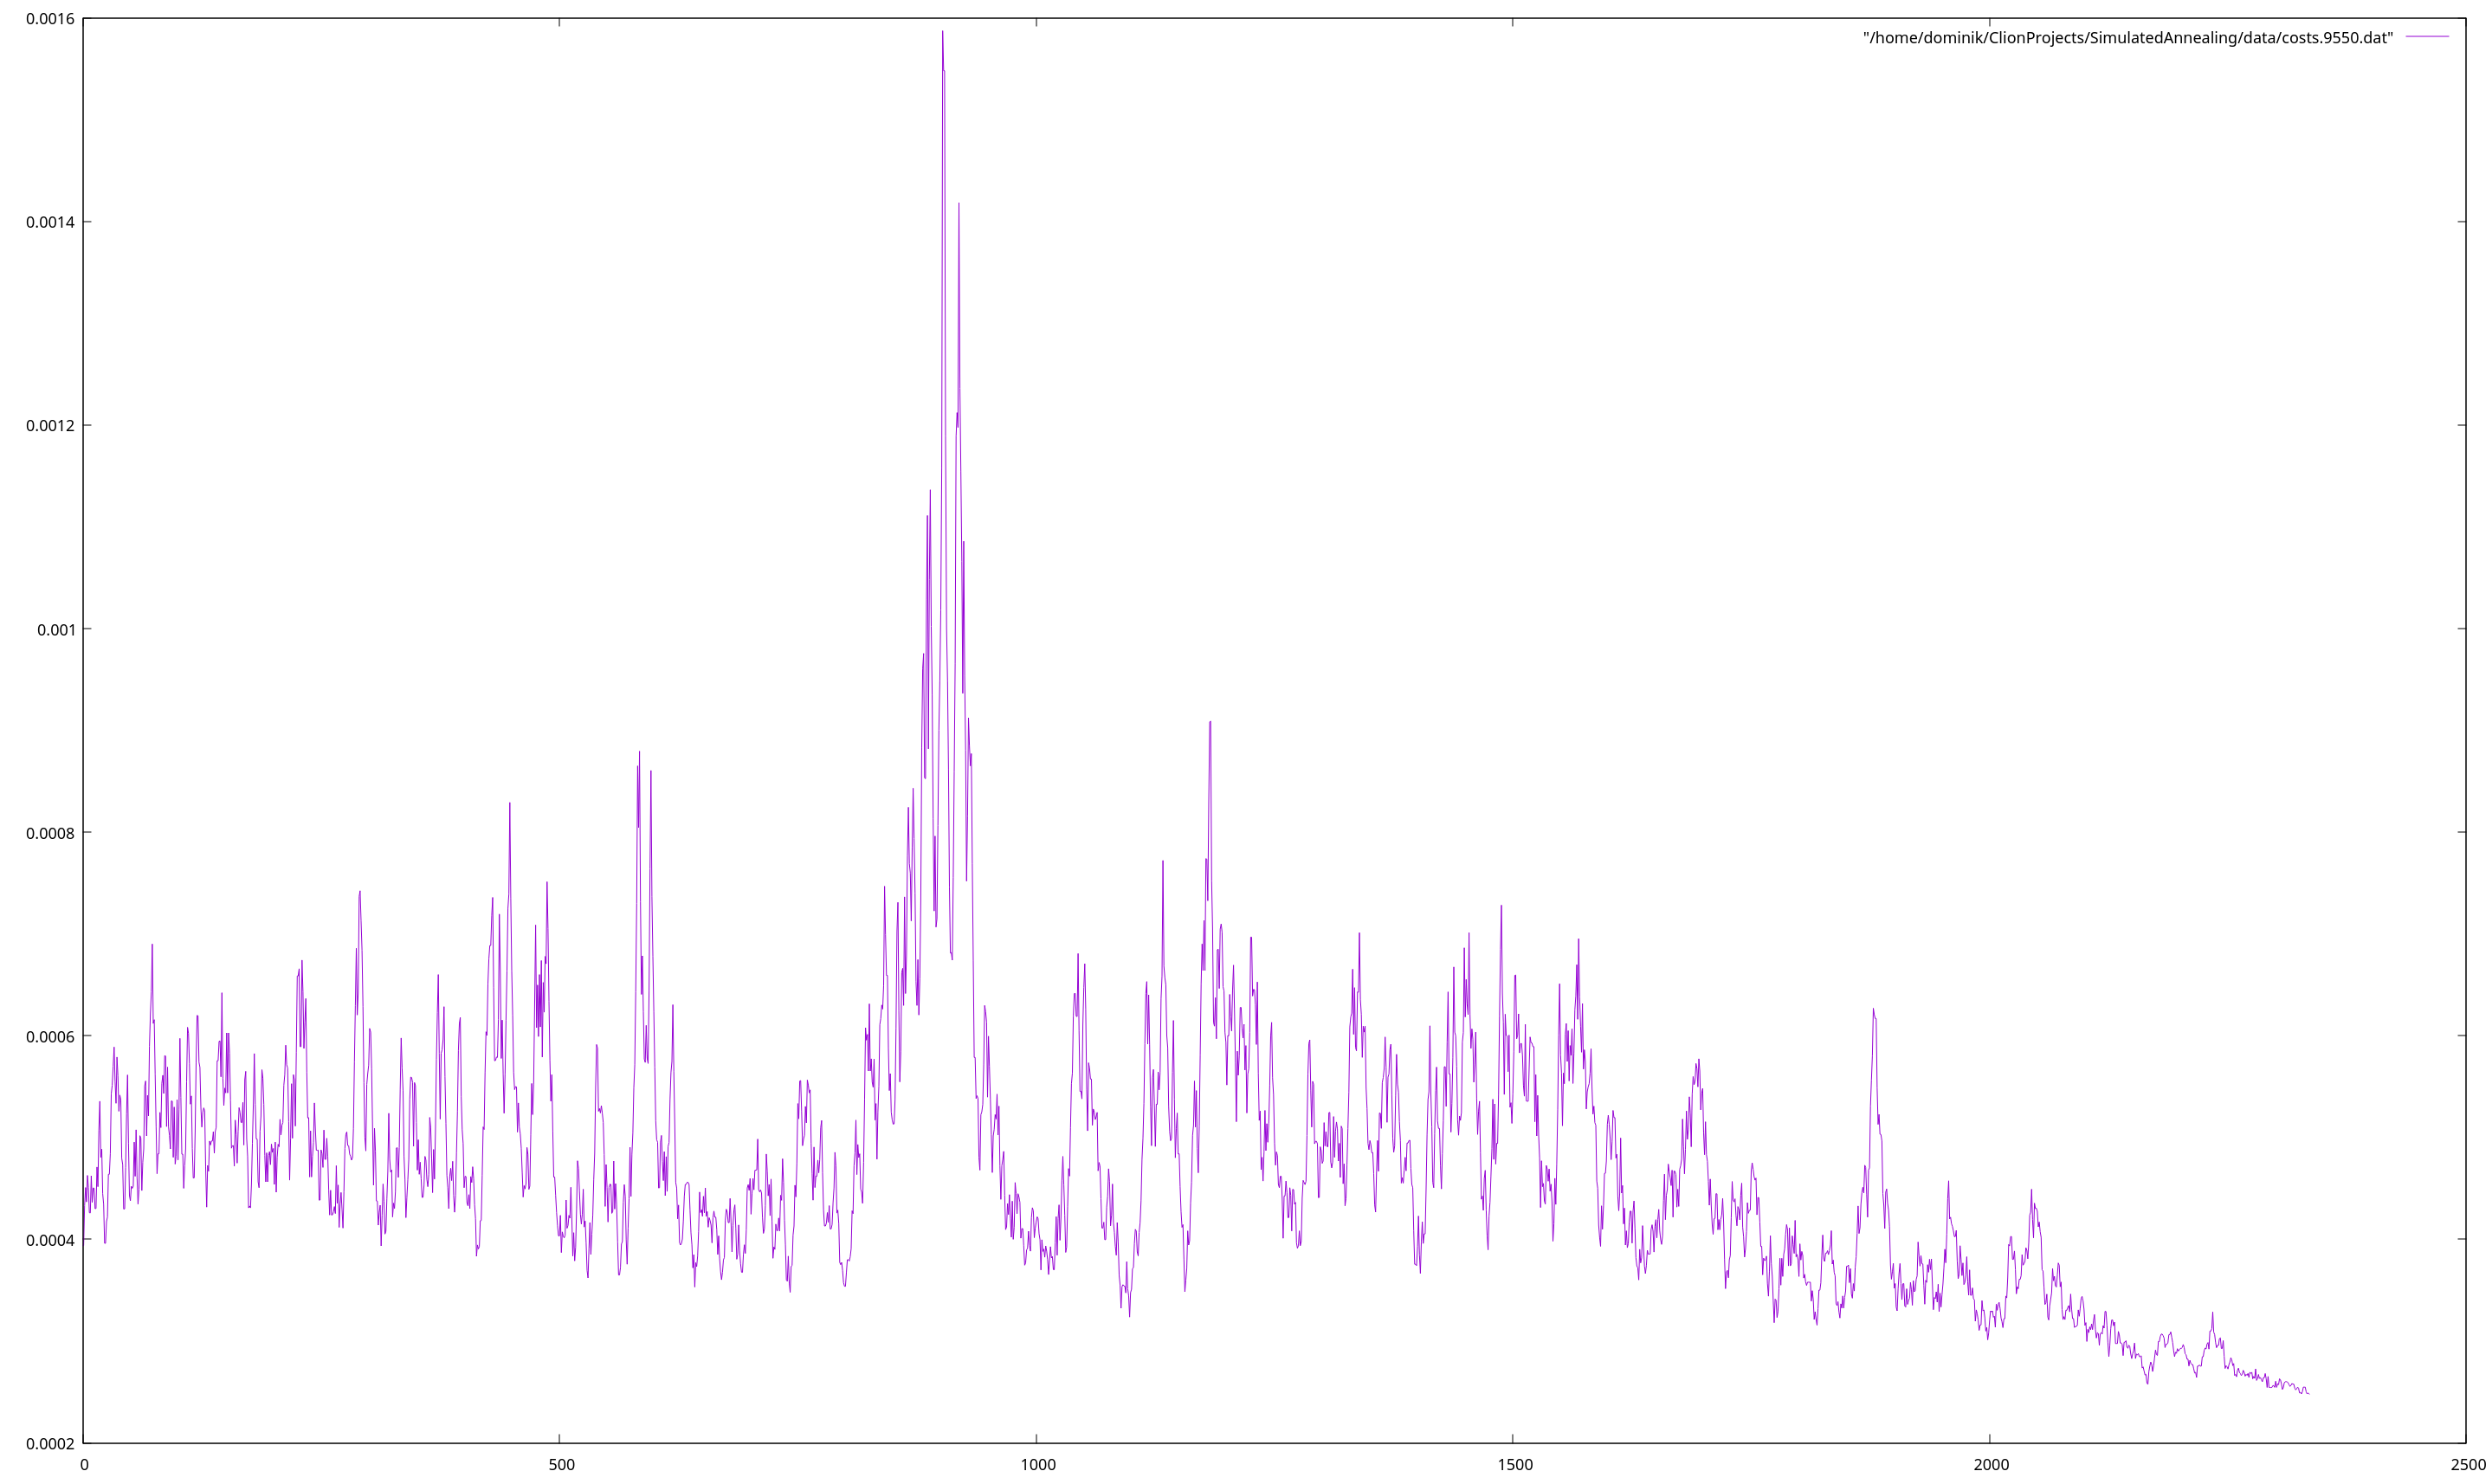
\includegraphics[width=\textwidth]{tooHighStart}
\caption{Příliš vysoká počáteční teplota - rel. chyba 0.0091}
\label{tooHighStart}
\end{figure}

\begin{figure}[H]
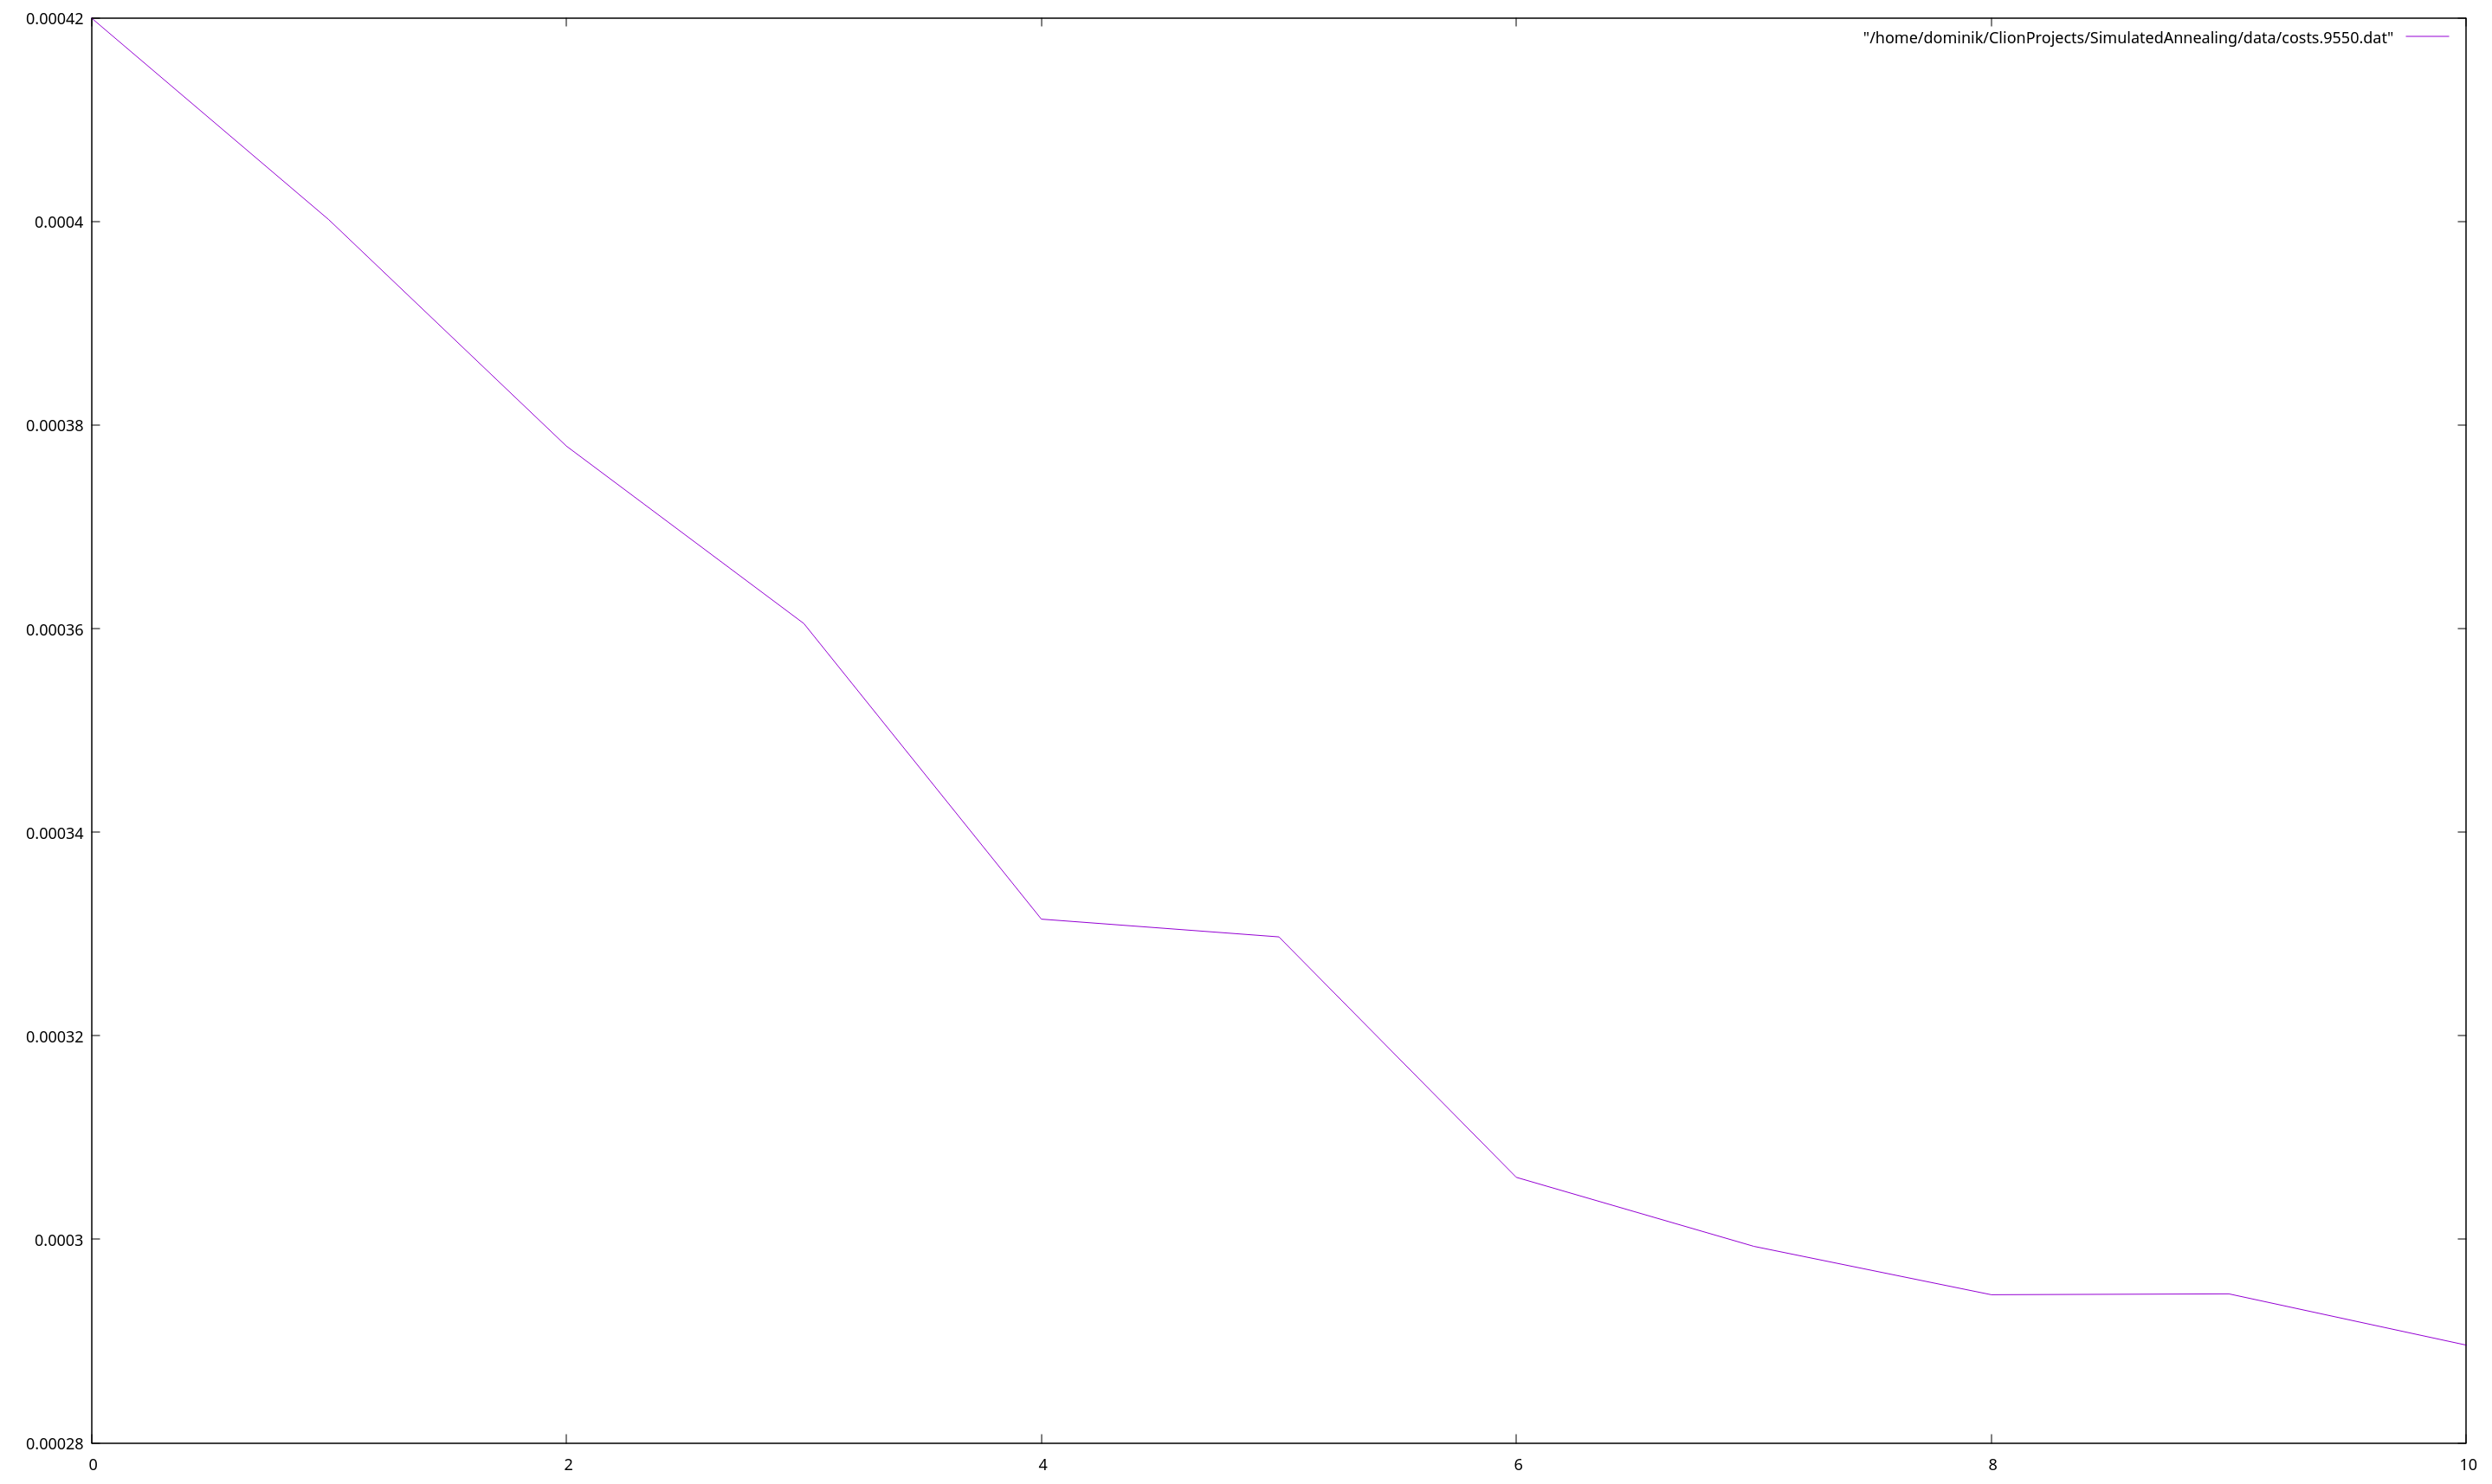
\includegraphics[width=\textwidth]{tooLowStart}
\caption{Příliš nízká počáteční teplota - rel. chyba 0.1512}
\label{tooLowStart}
\end{figure}

Dalším rozhodnutím je právě spodní mez teploty, tedy ta teplota, na níž se metoda zastaví. Tato opět lze volit fixně, ale může nastat problém, když zvolíme spodní hranici příliš vysoko. Metoda pak skončí dříve, než se dostane do fáze intensifikace, a vrátí málo optimální výsledek, jak je vidět na obrázku \ref{tooHighEnd}. Při příliš nízké koncové teplotě můžeme zbytečně dlouho čekat na výsledek, který se již nemění, viz obrázek \ref{tooLowEnd}.

\begin{figure}[H]
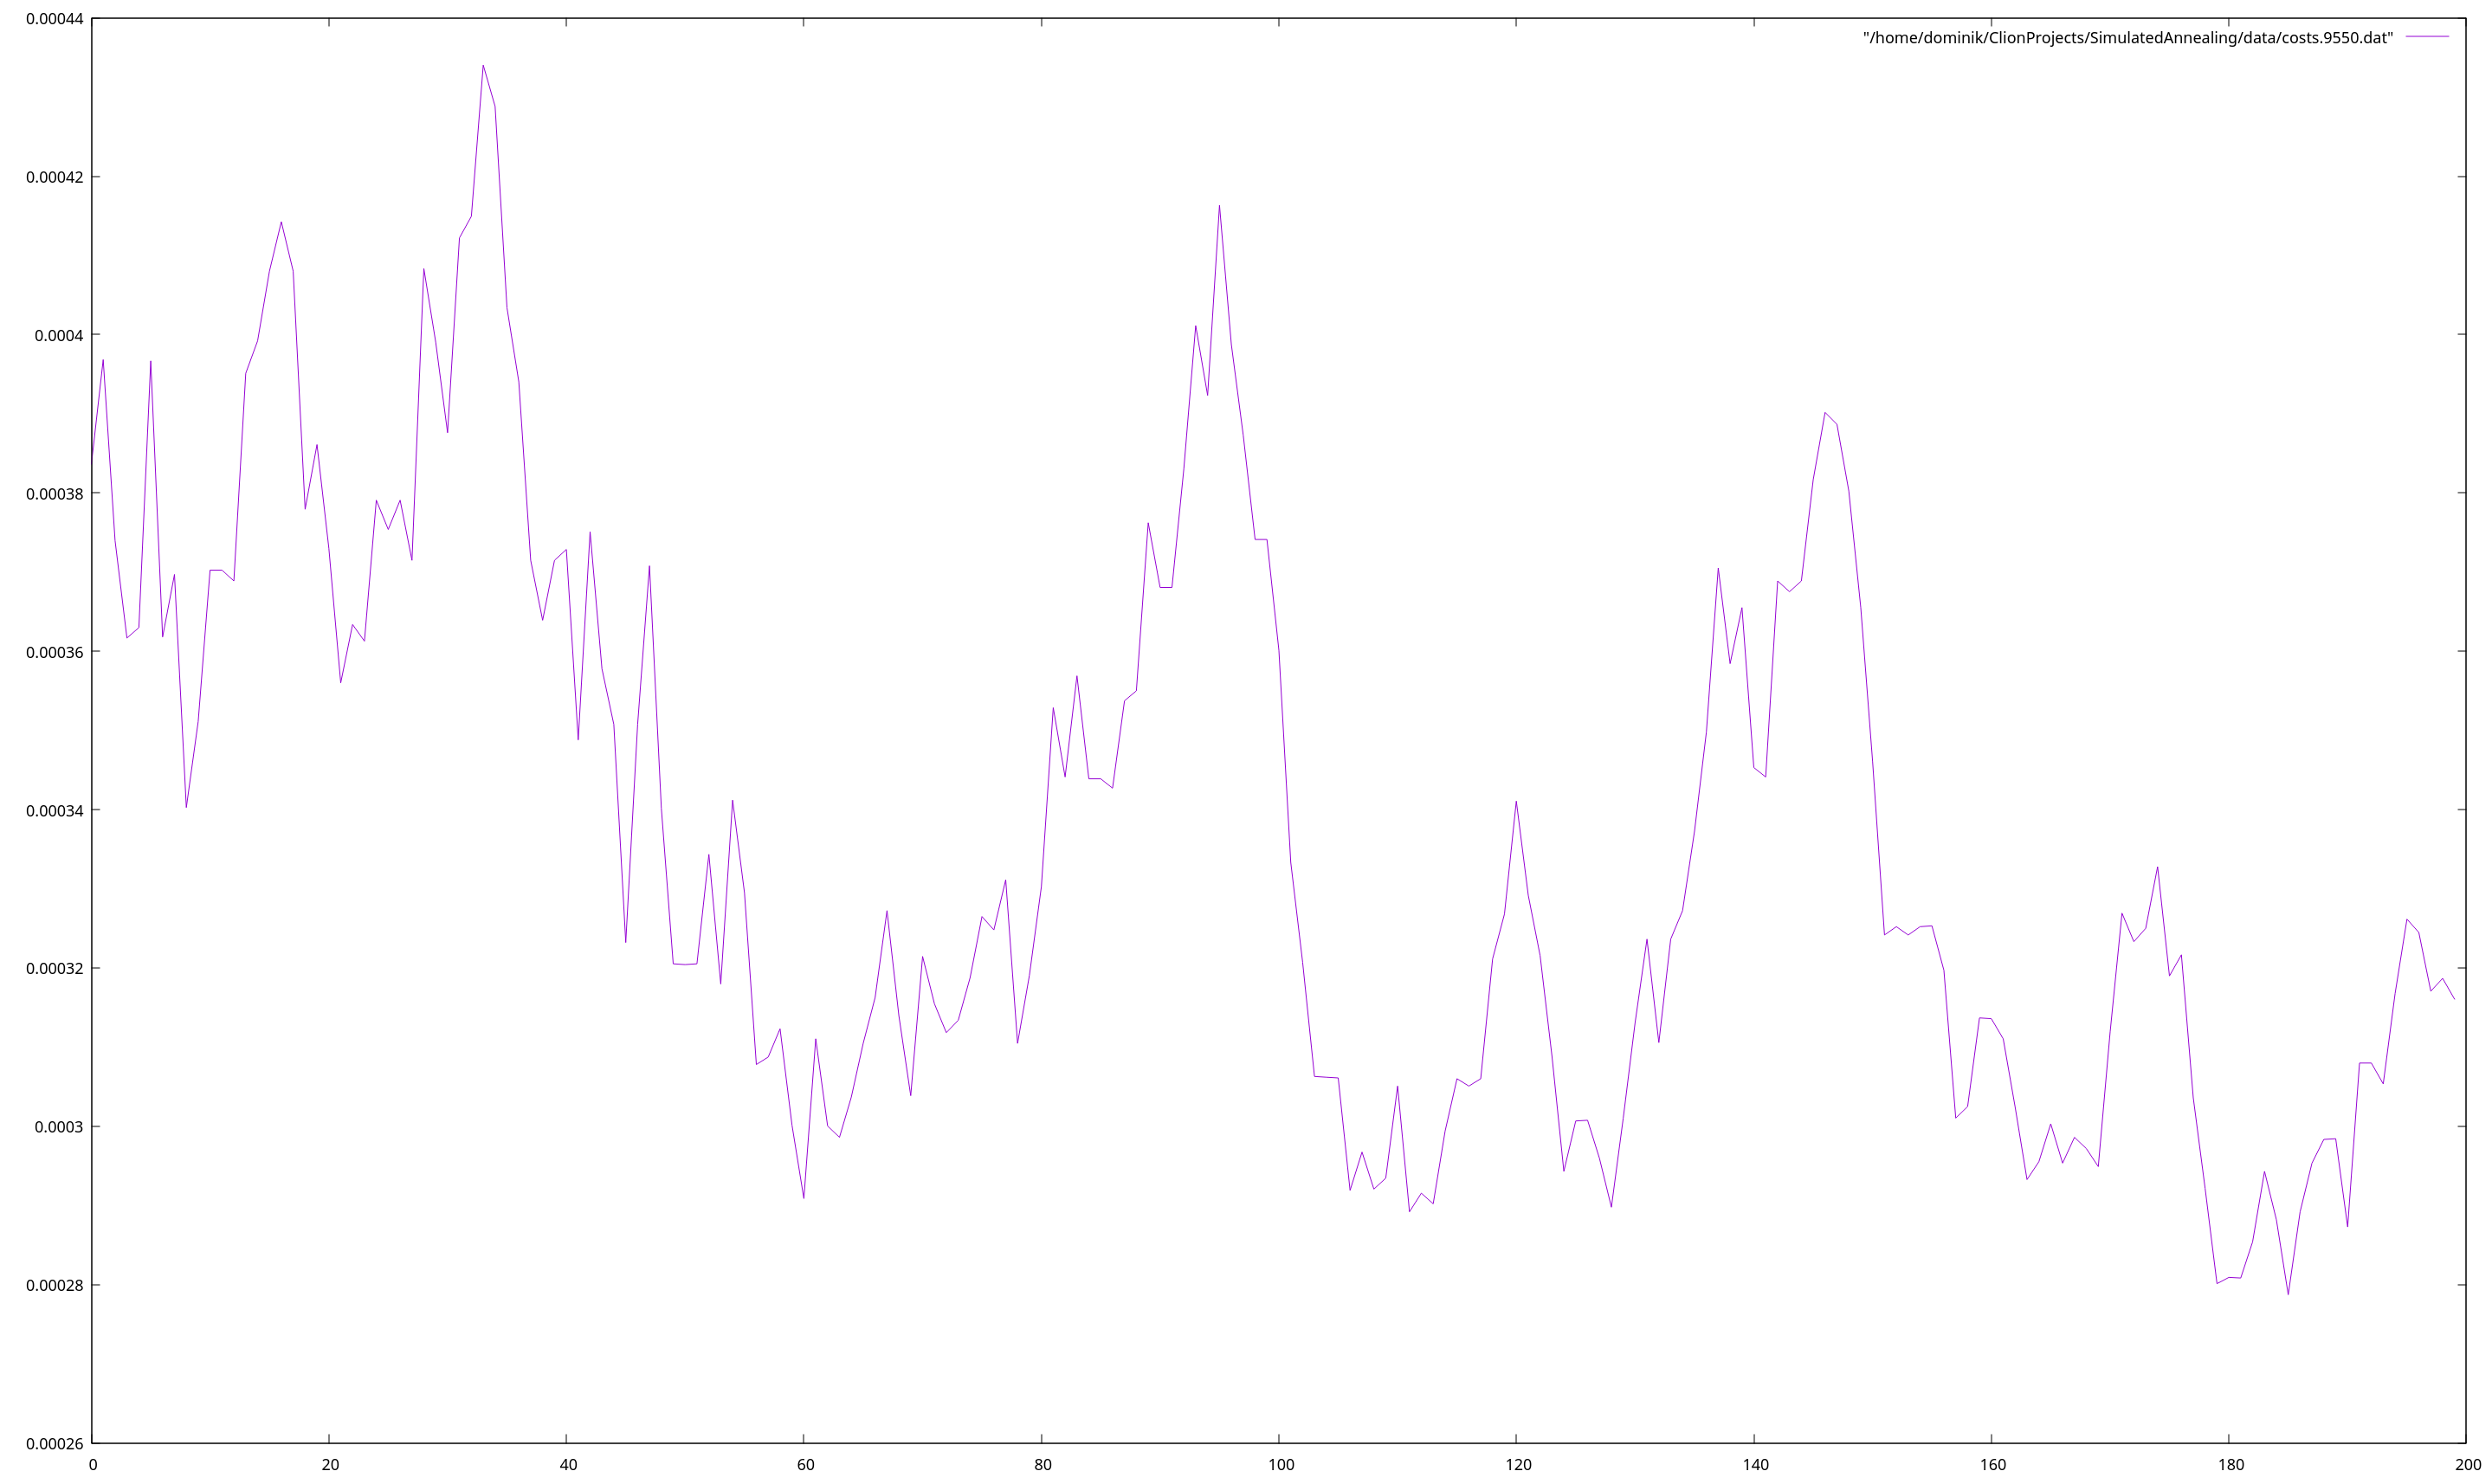
\includegraphics[width=\textwidth]{tooHighEnd}
\caption{Příliš vysoká koncová teplota - rel. chyba 0.1180}
\label{tooHighEnd}
\end{figure}

\begin{figure}[H]
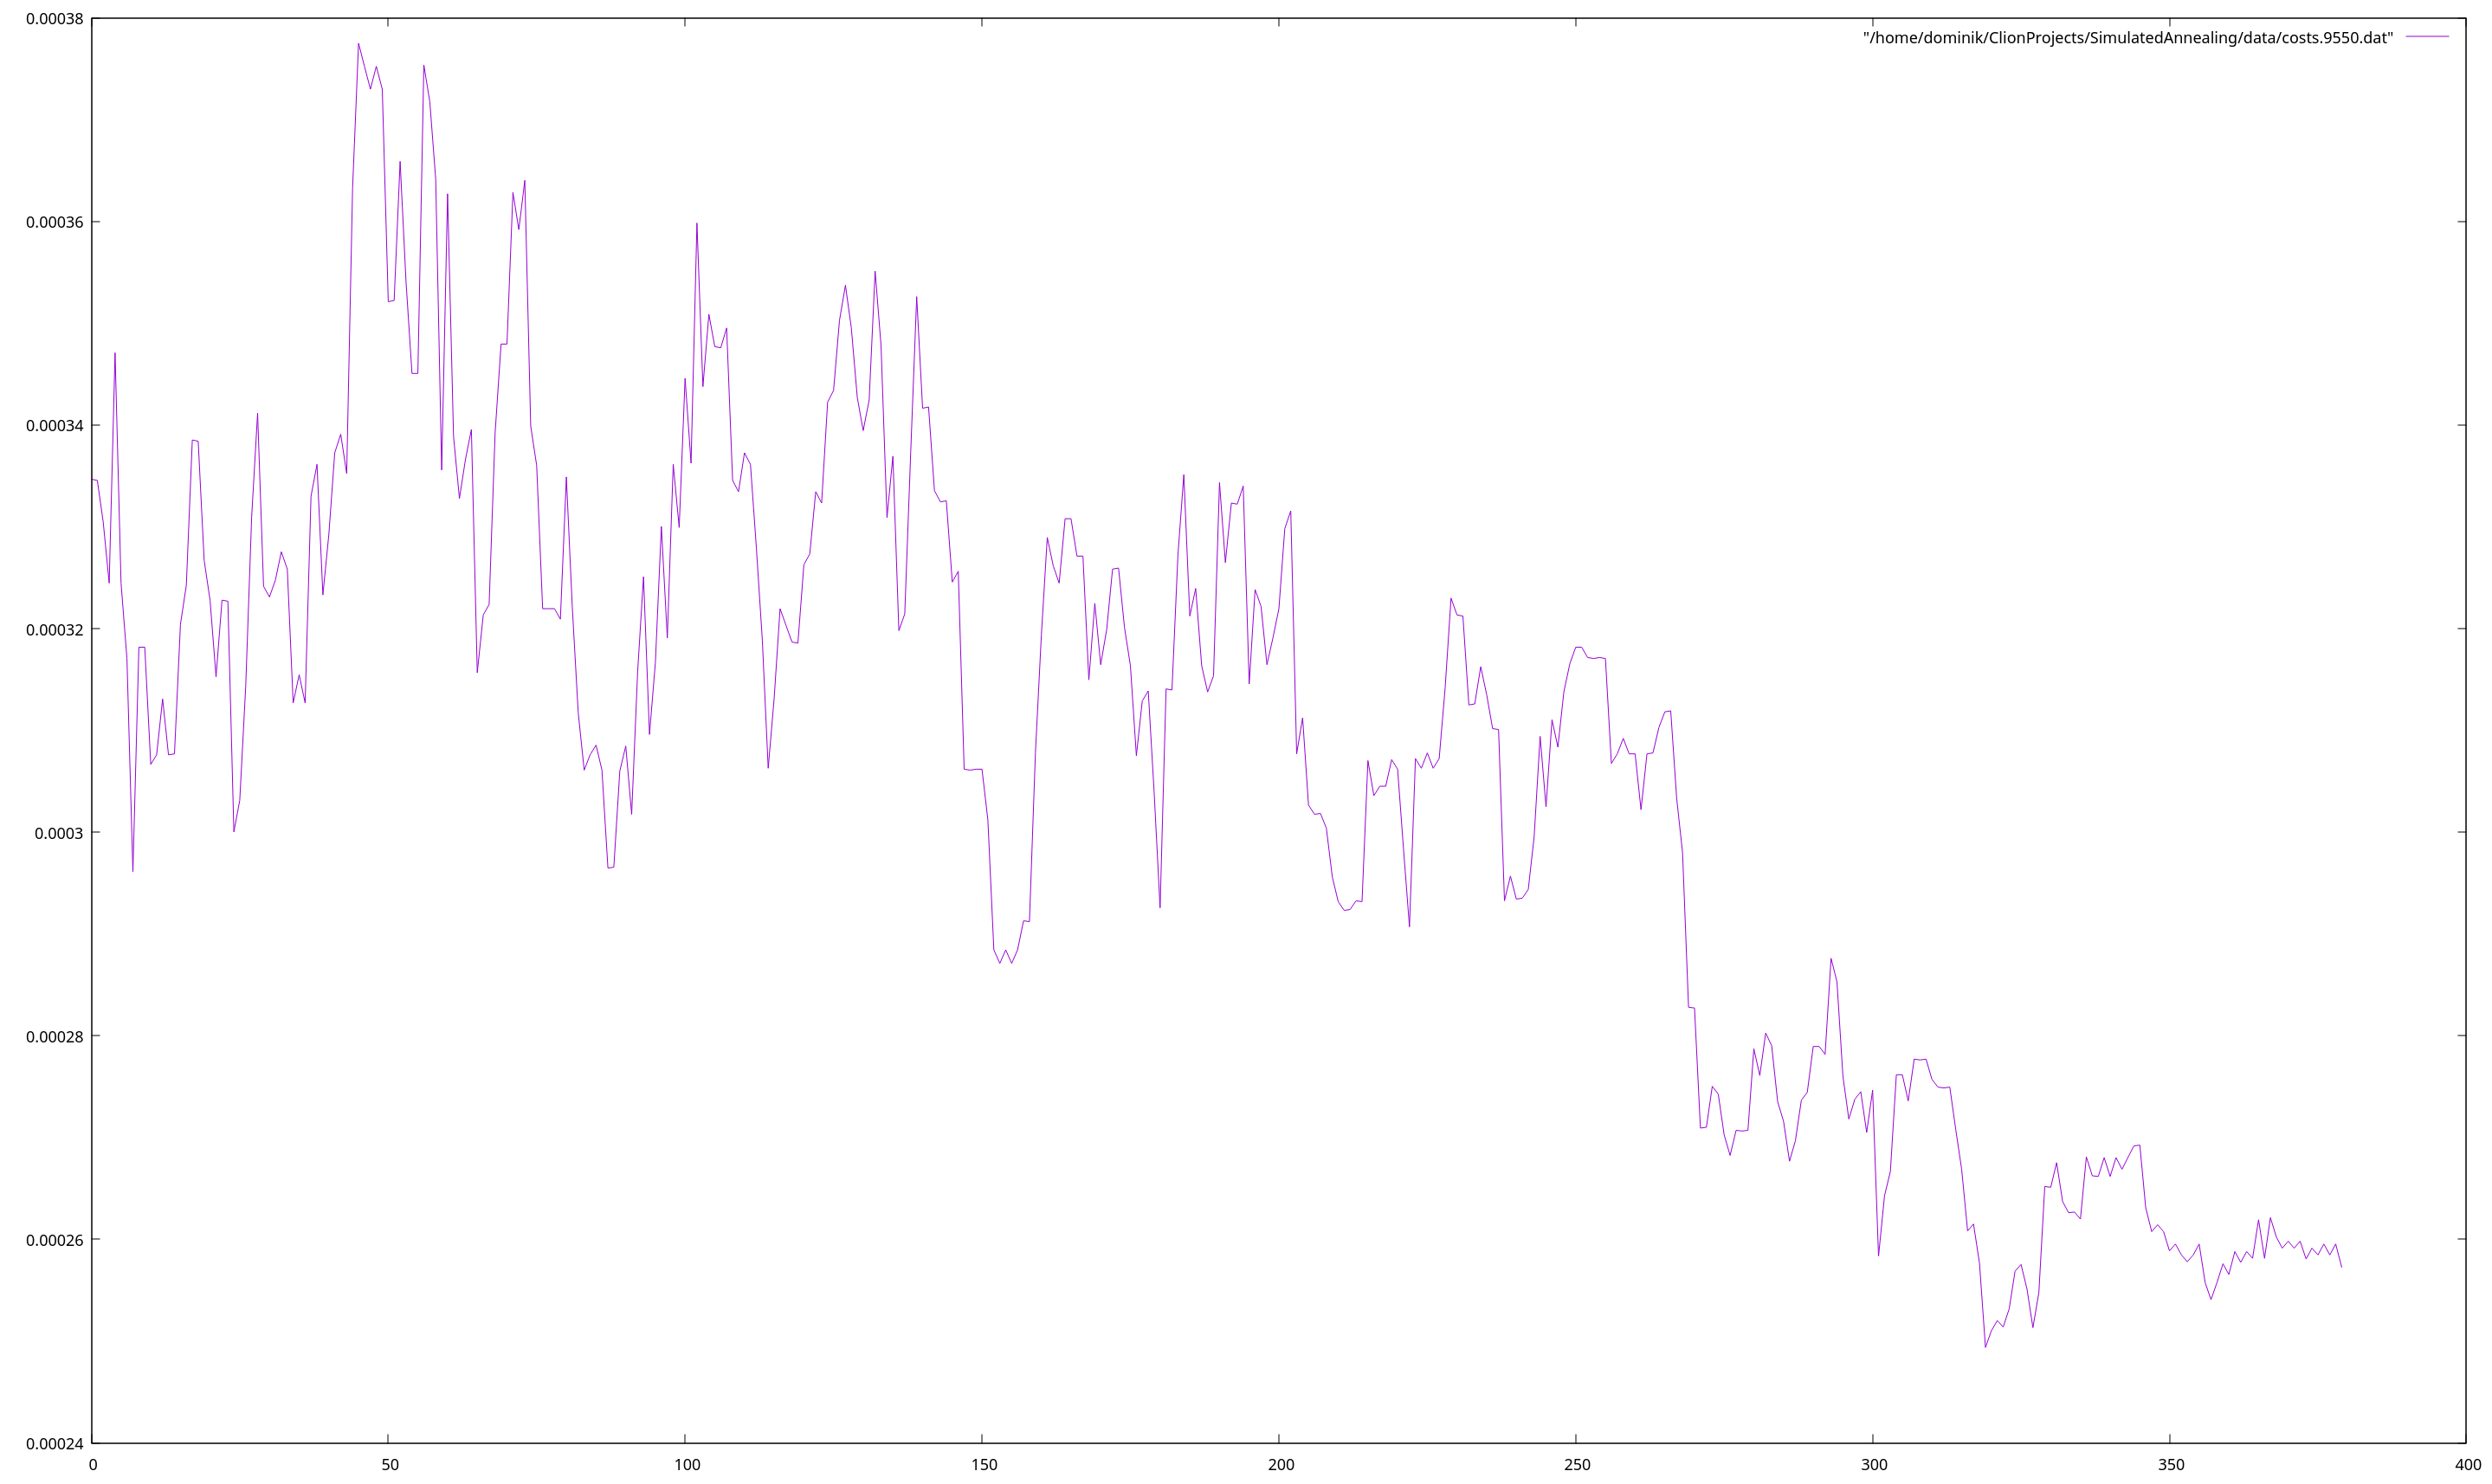
\includegraphics[width=\textwidth]{tooLowEnd}
\caption{Příliš nízká koncová teplota - rel. chyba 0.0143}
\label{tooLowEnd}
\end{figure}

\subsection{Sestavení počáteční teploty}
\label{startingTemp}

Počáteční teplota lze spočítat. Místo abychom ji hádali, spustíme nejdříve ,,metodu prudkého ohřívání``. Ta začne na velmi nízké počáteční teplotě a rychle ji zvyšuje. Jakmile je dosaženo teploty, kdy je poloviční pravděpodobnost, že je přijat jako další stav stav horší, zaznamenáme tuto teplotu jako počáteční, a teprve potom spouštíme normální běh metody.

Tento postup jsem se rozhodl implementovat. Za rychlost ohřívání jsem zvolil parametr 1.5. Pro každou teplotu se spočítá počet přijatých skoků do sousedního stavu a kolik z nich jsou skoky k horšímu. Jakmile tento poměr dosáhne poloviny, zastaví se příprava, zaznamená se teplota a hlavní průběh metody se spustí s touto počáteční teplotou.

\subsection{Zmrznutí}
\label{freeze}

Koncová teplota lze též volit dynamicky. Lze počítat, kolik skoků se algoritmus rozhodl provést ze všech nabízených (ovšem jen takových, pro které není přesažena kapacita batohu, ty jsou ignorovány).

V mém případě metoda tento poměr spočítá pro každou testovanou teplotu a dostáne-li méně než 5\%, dojde ke ,,zmrznutí`` a metoda končí.


\section{Měření}

\subsection{Detail pěti průběhů}

Za použití dynamického určení počáteční i koncové teploty jsem se rozhodl sledovat průběh metody na výše uvedené instanci postupně pro pět různých hodnot parametru rychlosti ochlazování, od 0,80 až po 0,99. Vyšší číslo znamená pomalejší pokles teploty a pravděpodobně i delší dobu trvání metody.

Různé průběhy jsou znázorněny na obrázcích \ref{topCalcBottomCalc80}, \ref{topCalcBottomCalc85}, \ref{topCalcBottomCalc90}, \ref{topCalcBottomCalc95} a \ref{topCalcBottomCalc99}.


\begin{figure}[H]
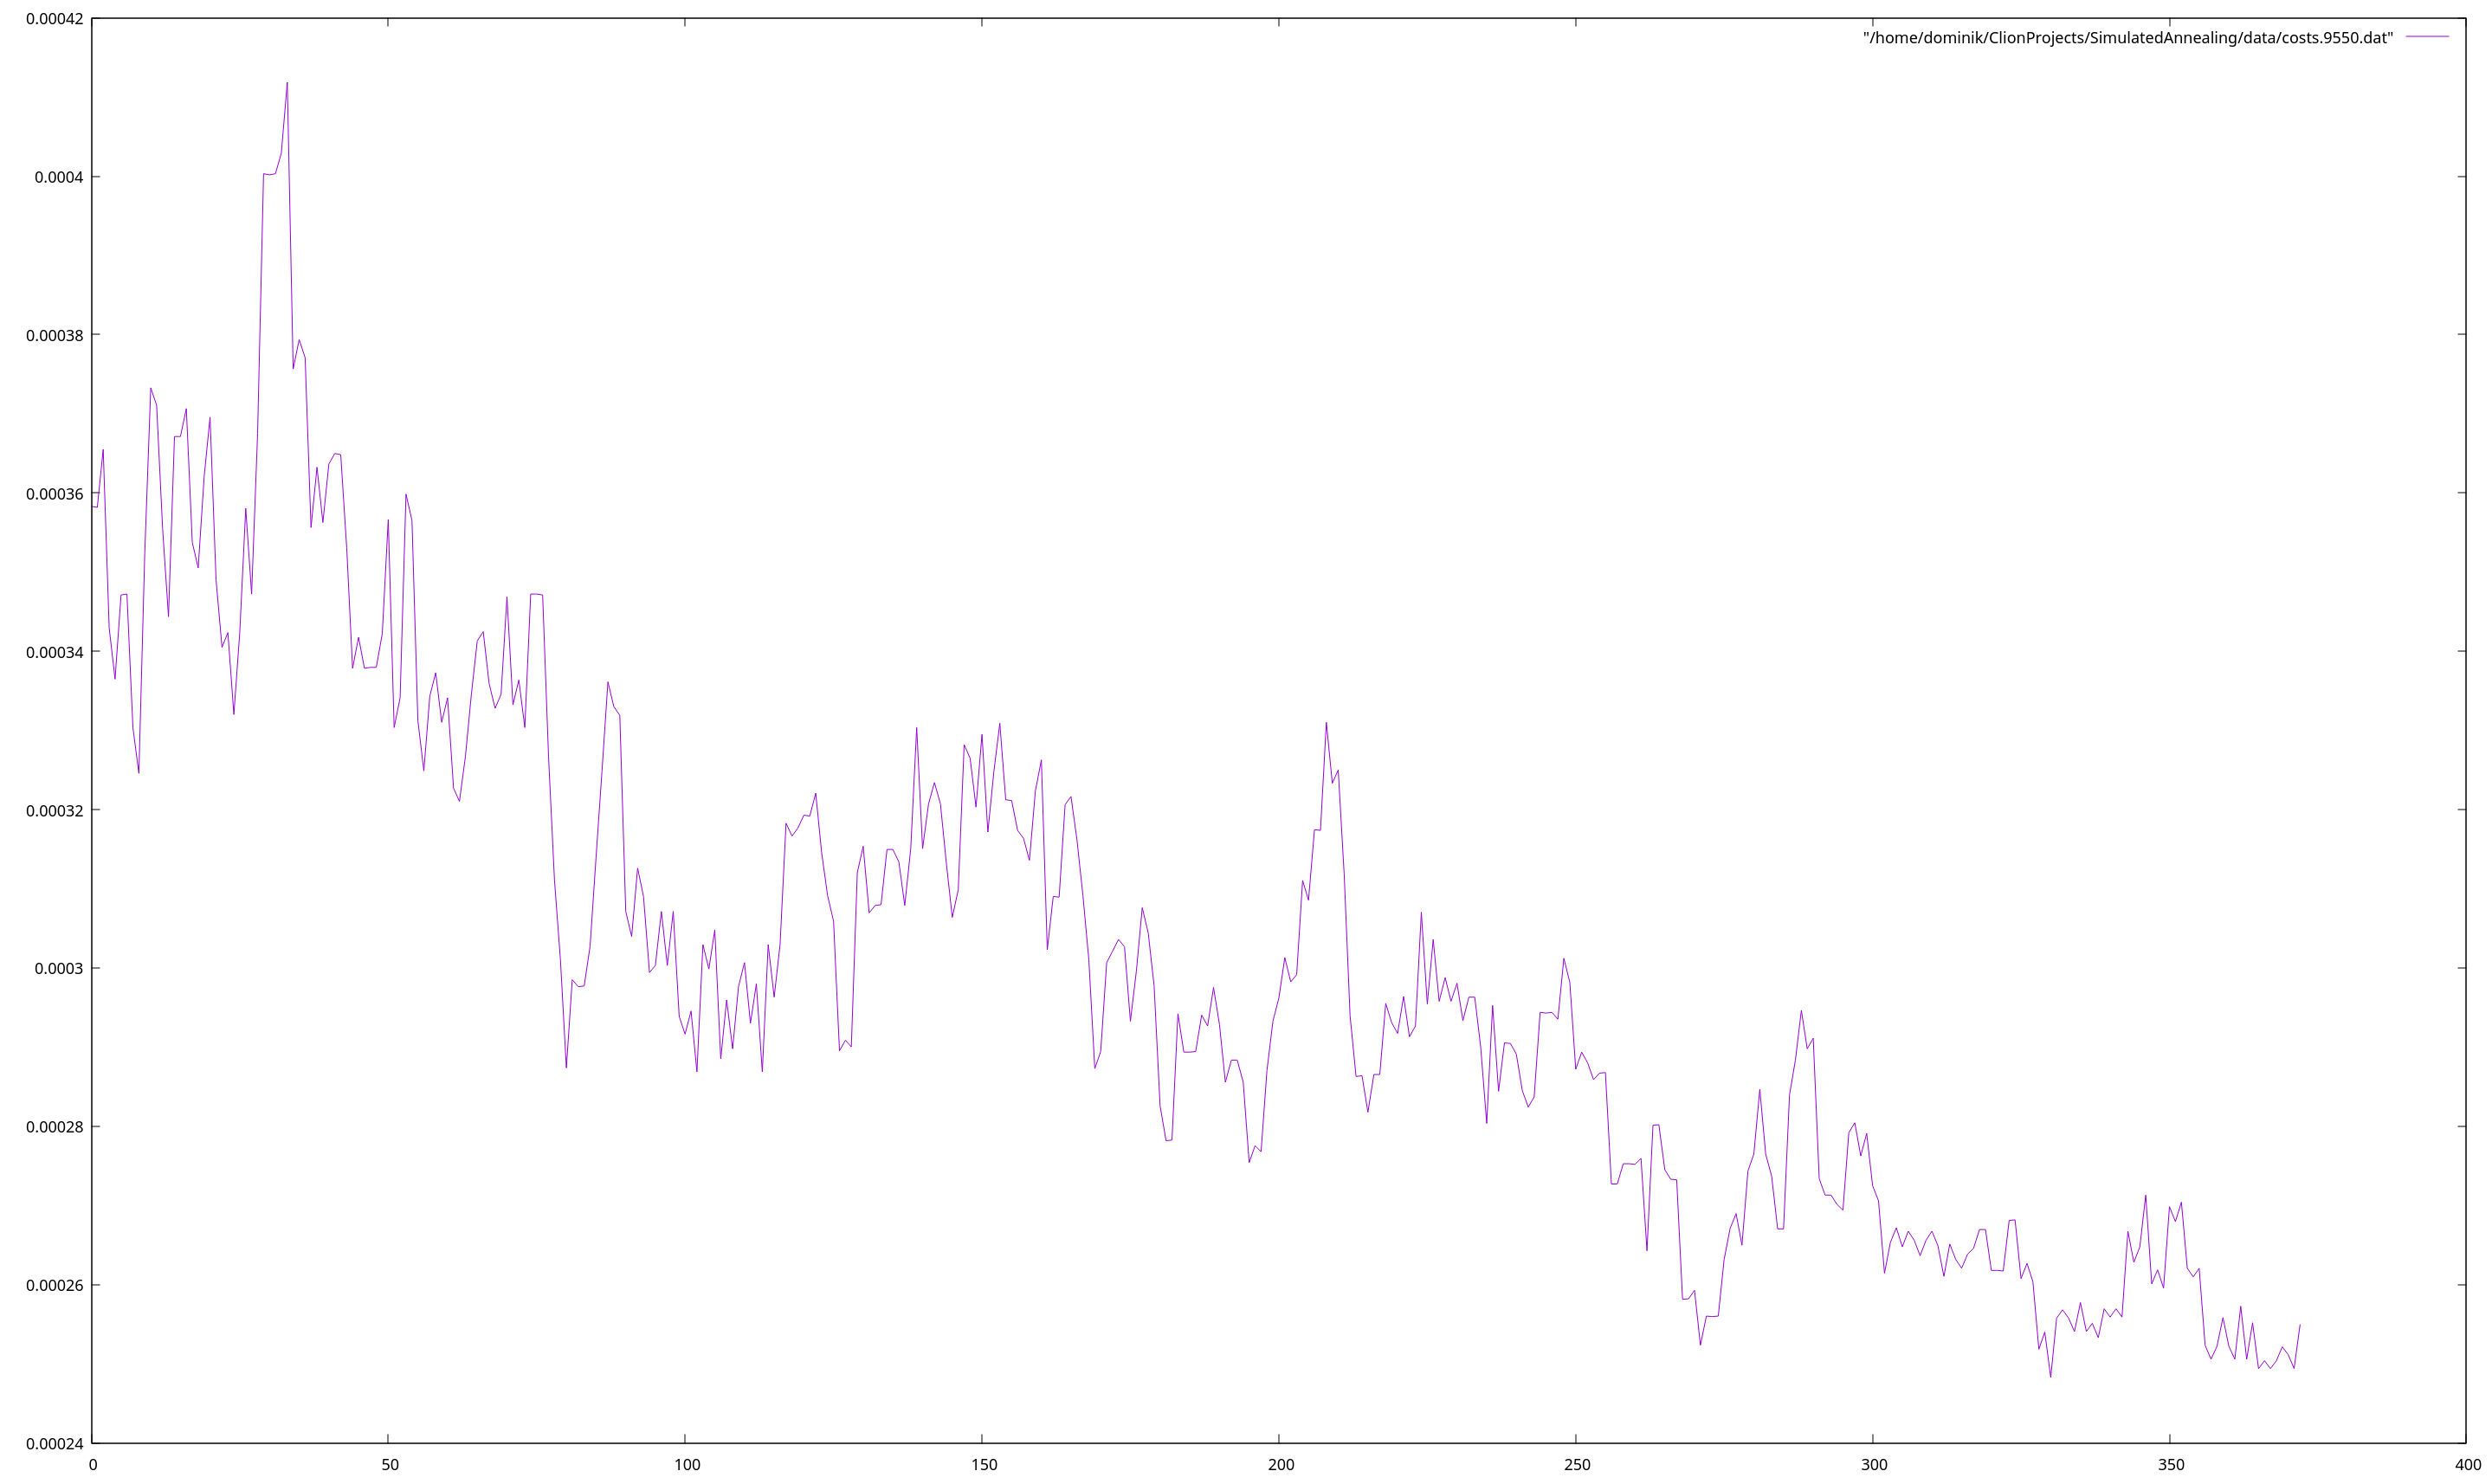
\includegraphics[width=\textwidth]{topCalcBottomCalc80}
\caption{Rychlost ochlazování 0,80 - rel. chyba 0.0054}
\label{topCalcBottomCalc80}
\end{figure}

\begin{figure}[H]
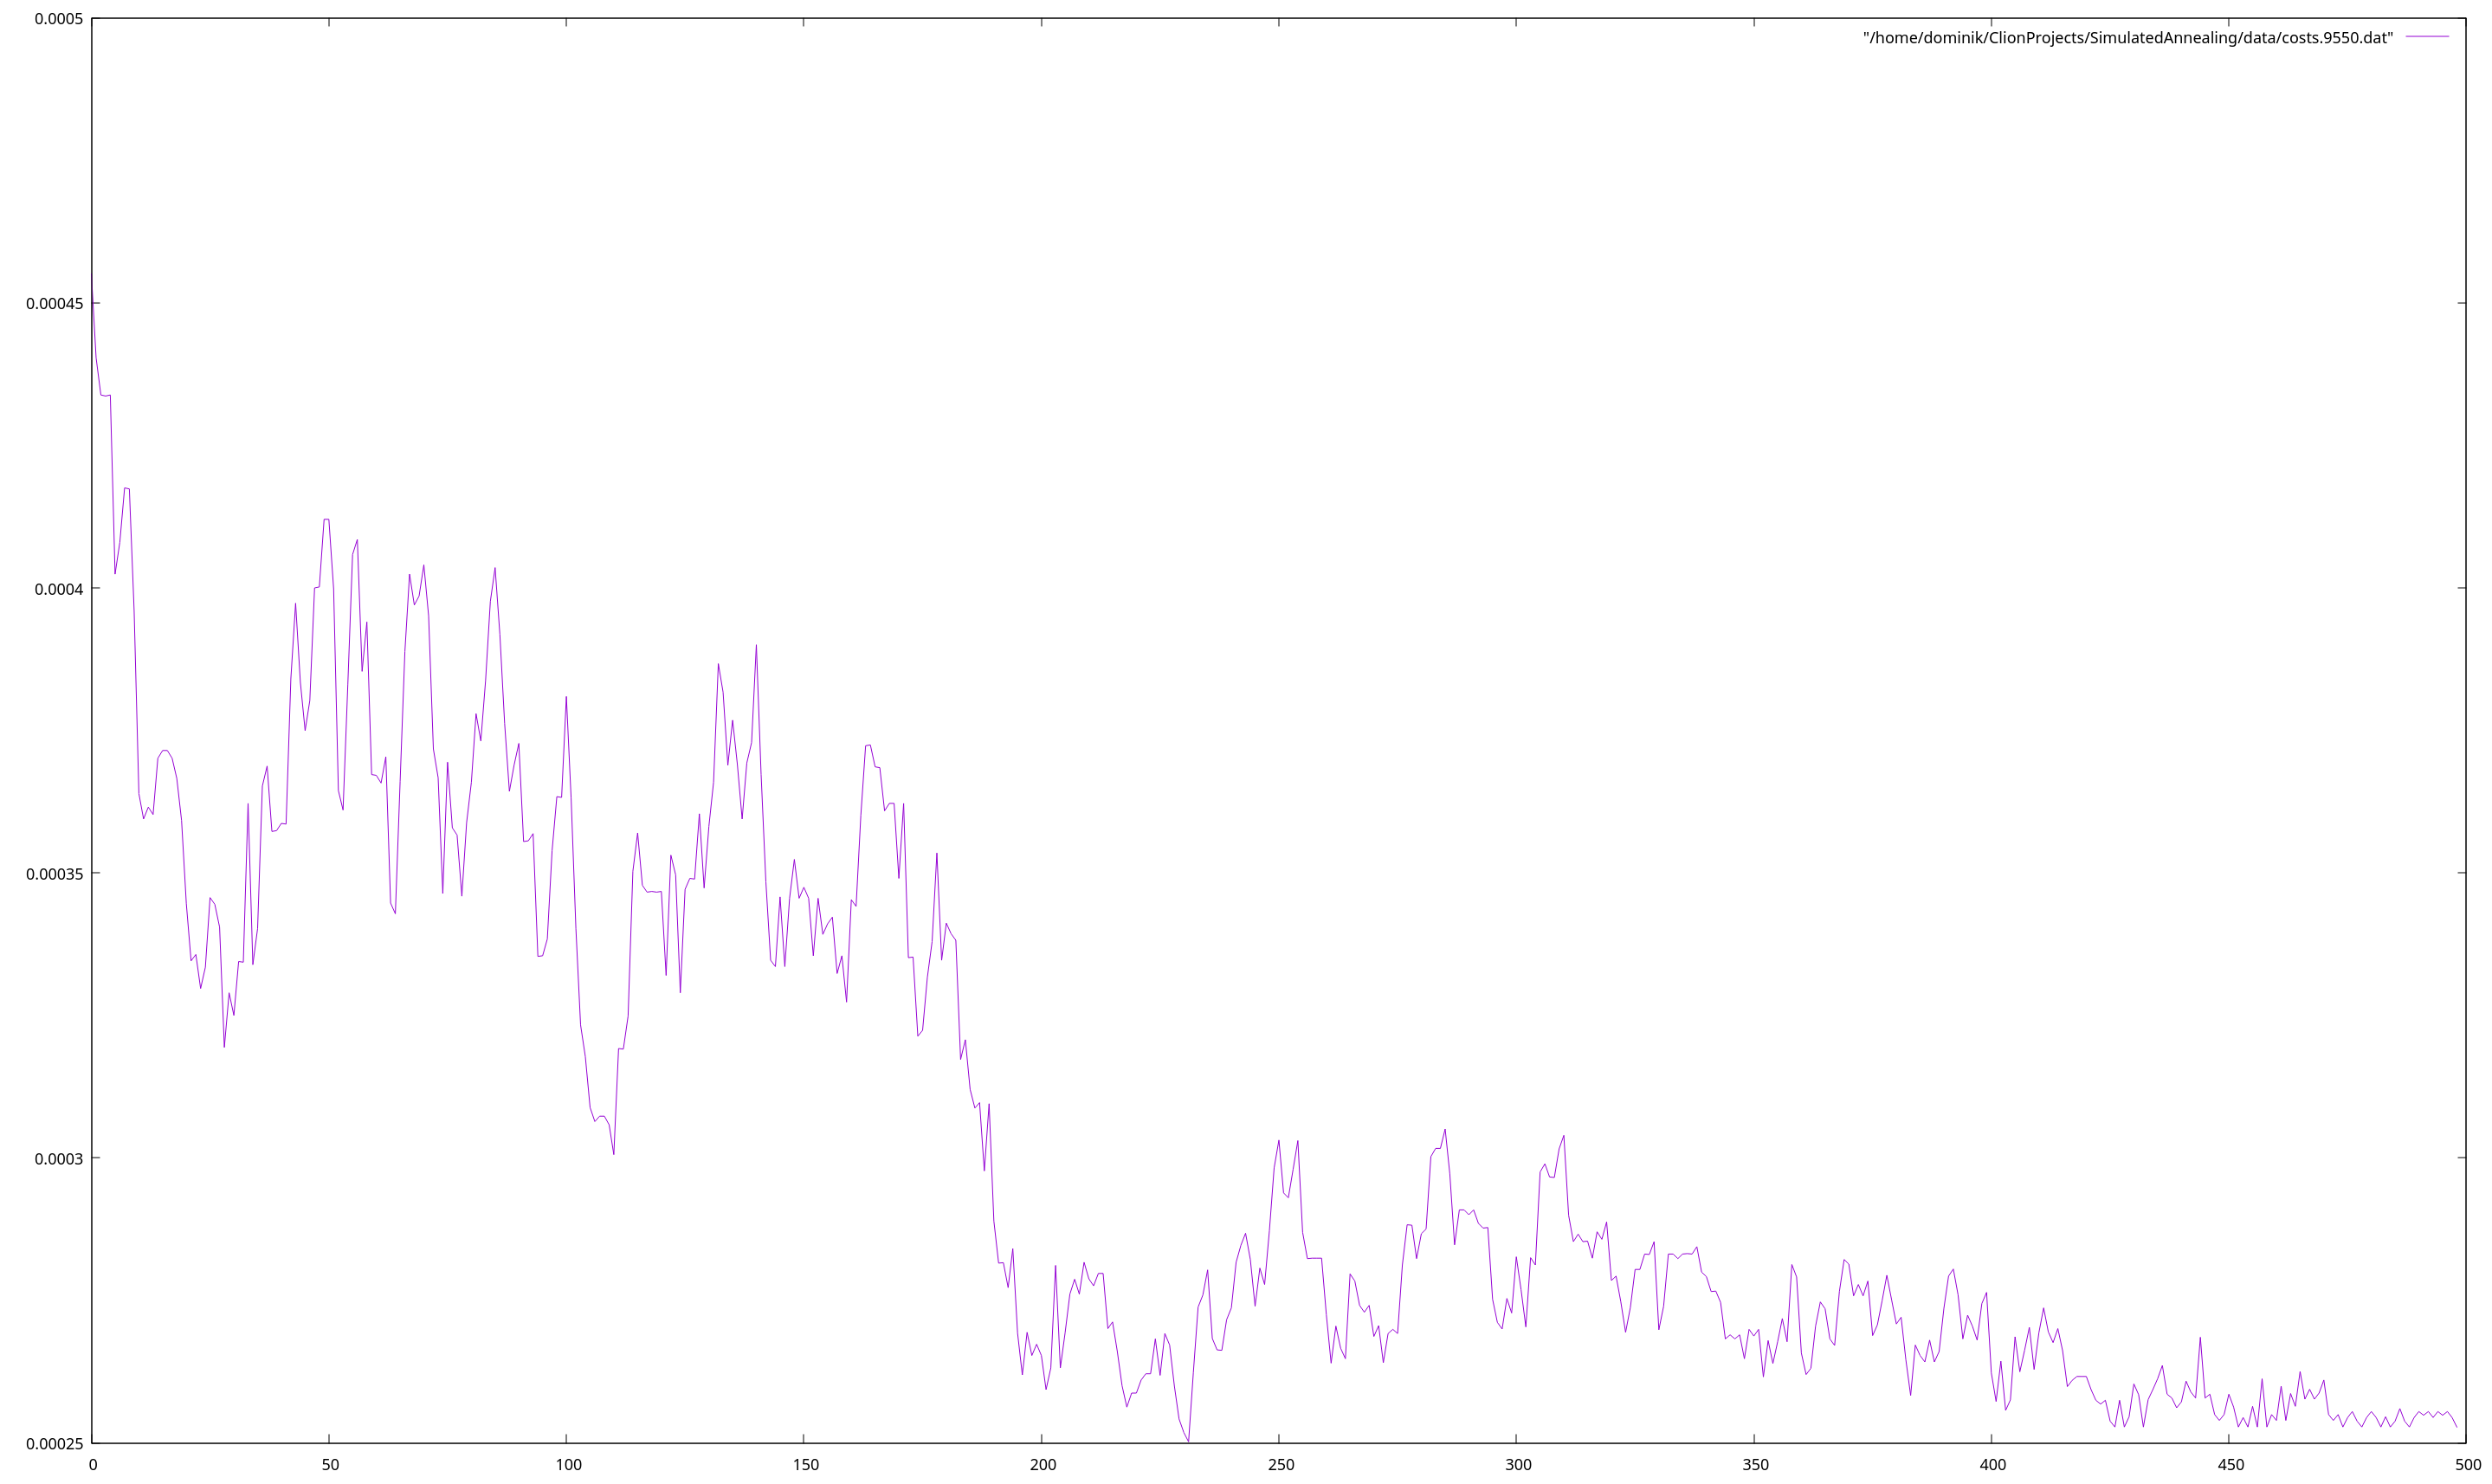
\includegraphics[width=\textwidth]{topCalcBottomCalc85}
\caption{Rychlost ochlazování 0,85 - rel. chyba 0.01745}
\label{topCalcBottomCalc85}
\end{figure}

\begin{figure}[H]
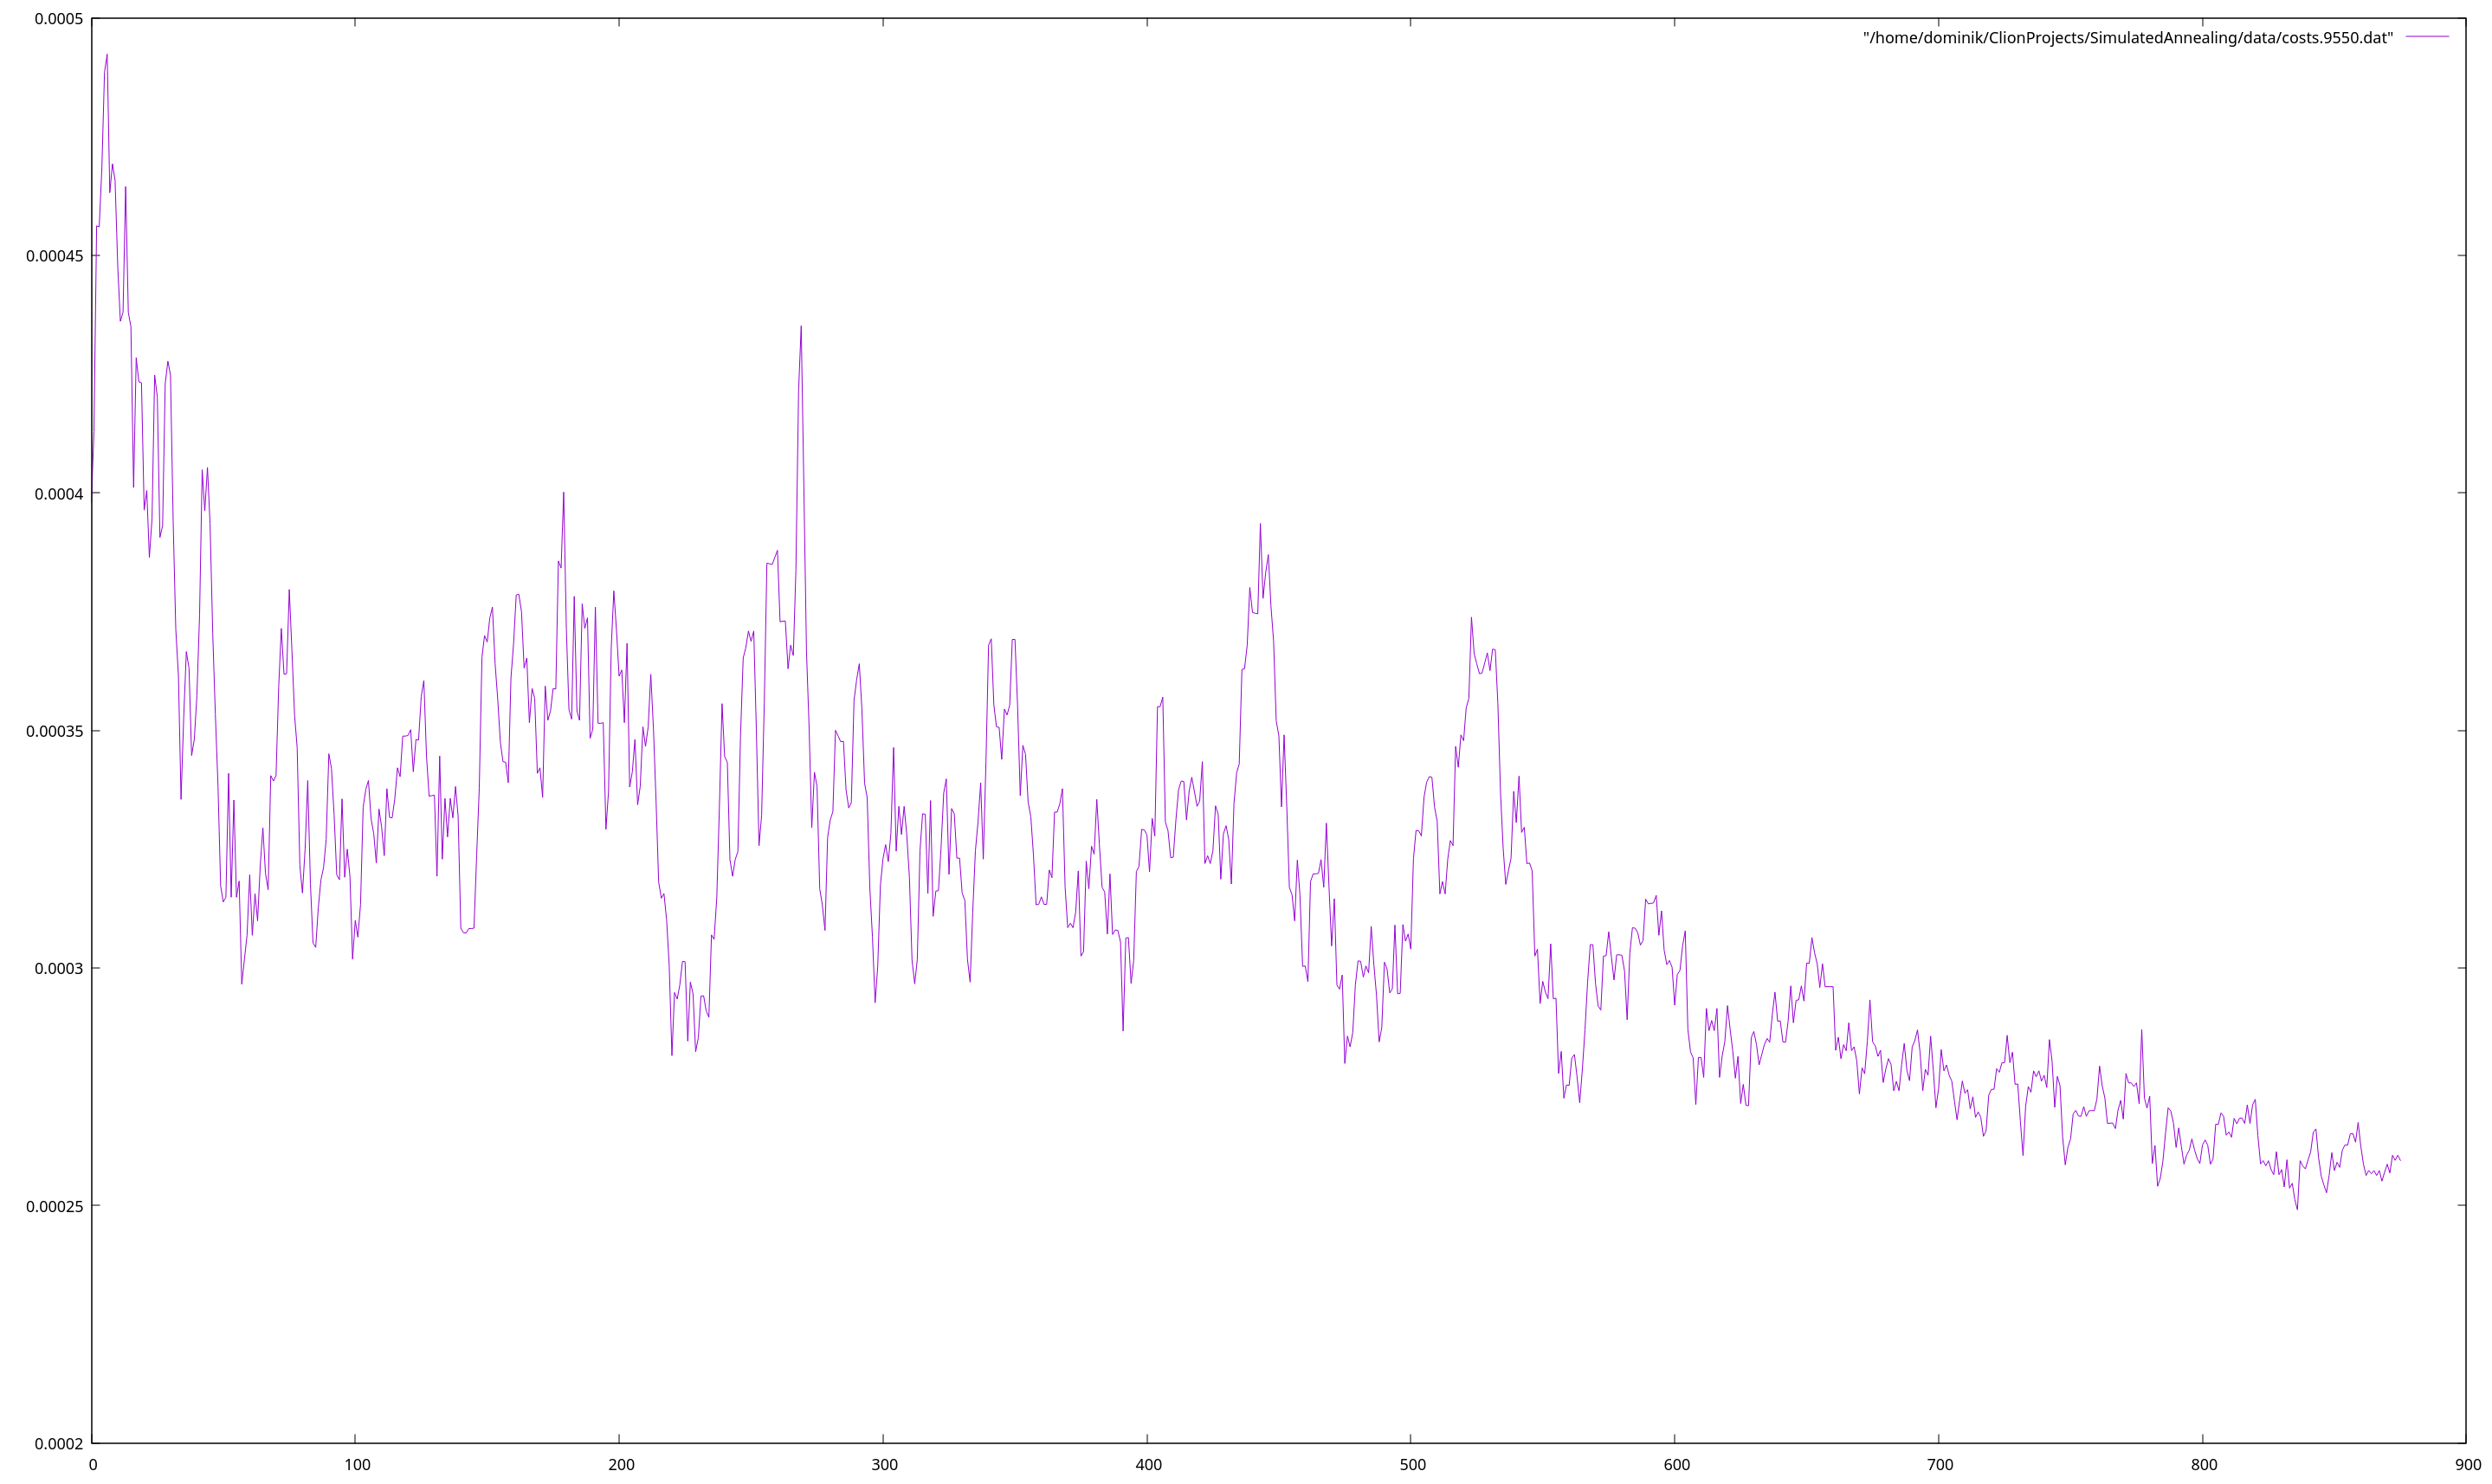
\includegraphics[width=\textwidth]{topCalcBottomCalc90}
\caption{Rychlost ochlazování 0,90 - rel. chyba 0.01302}
\label{topCalcBottomCalc90}
\end{figure}

\begin{figure}[H]
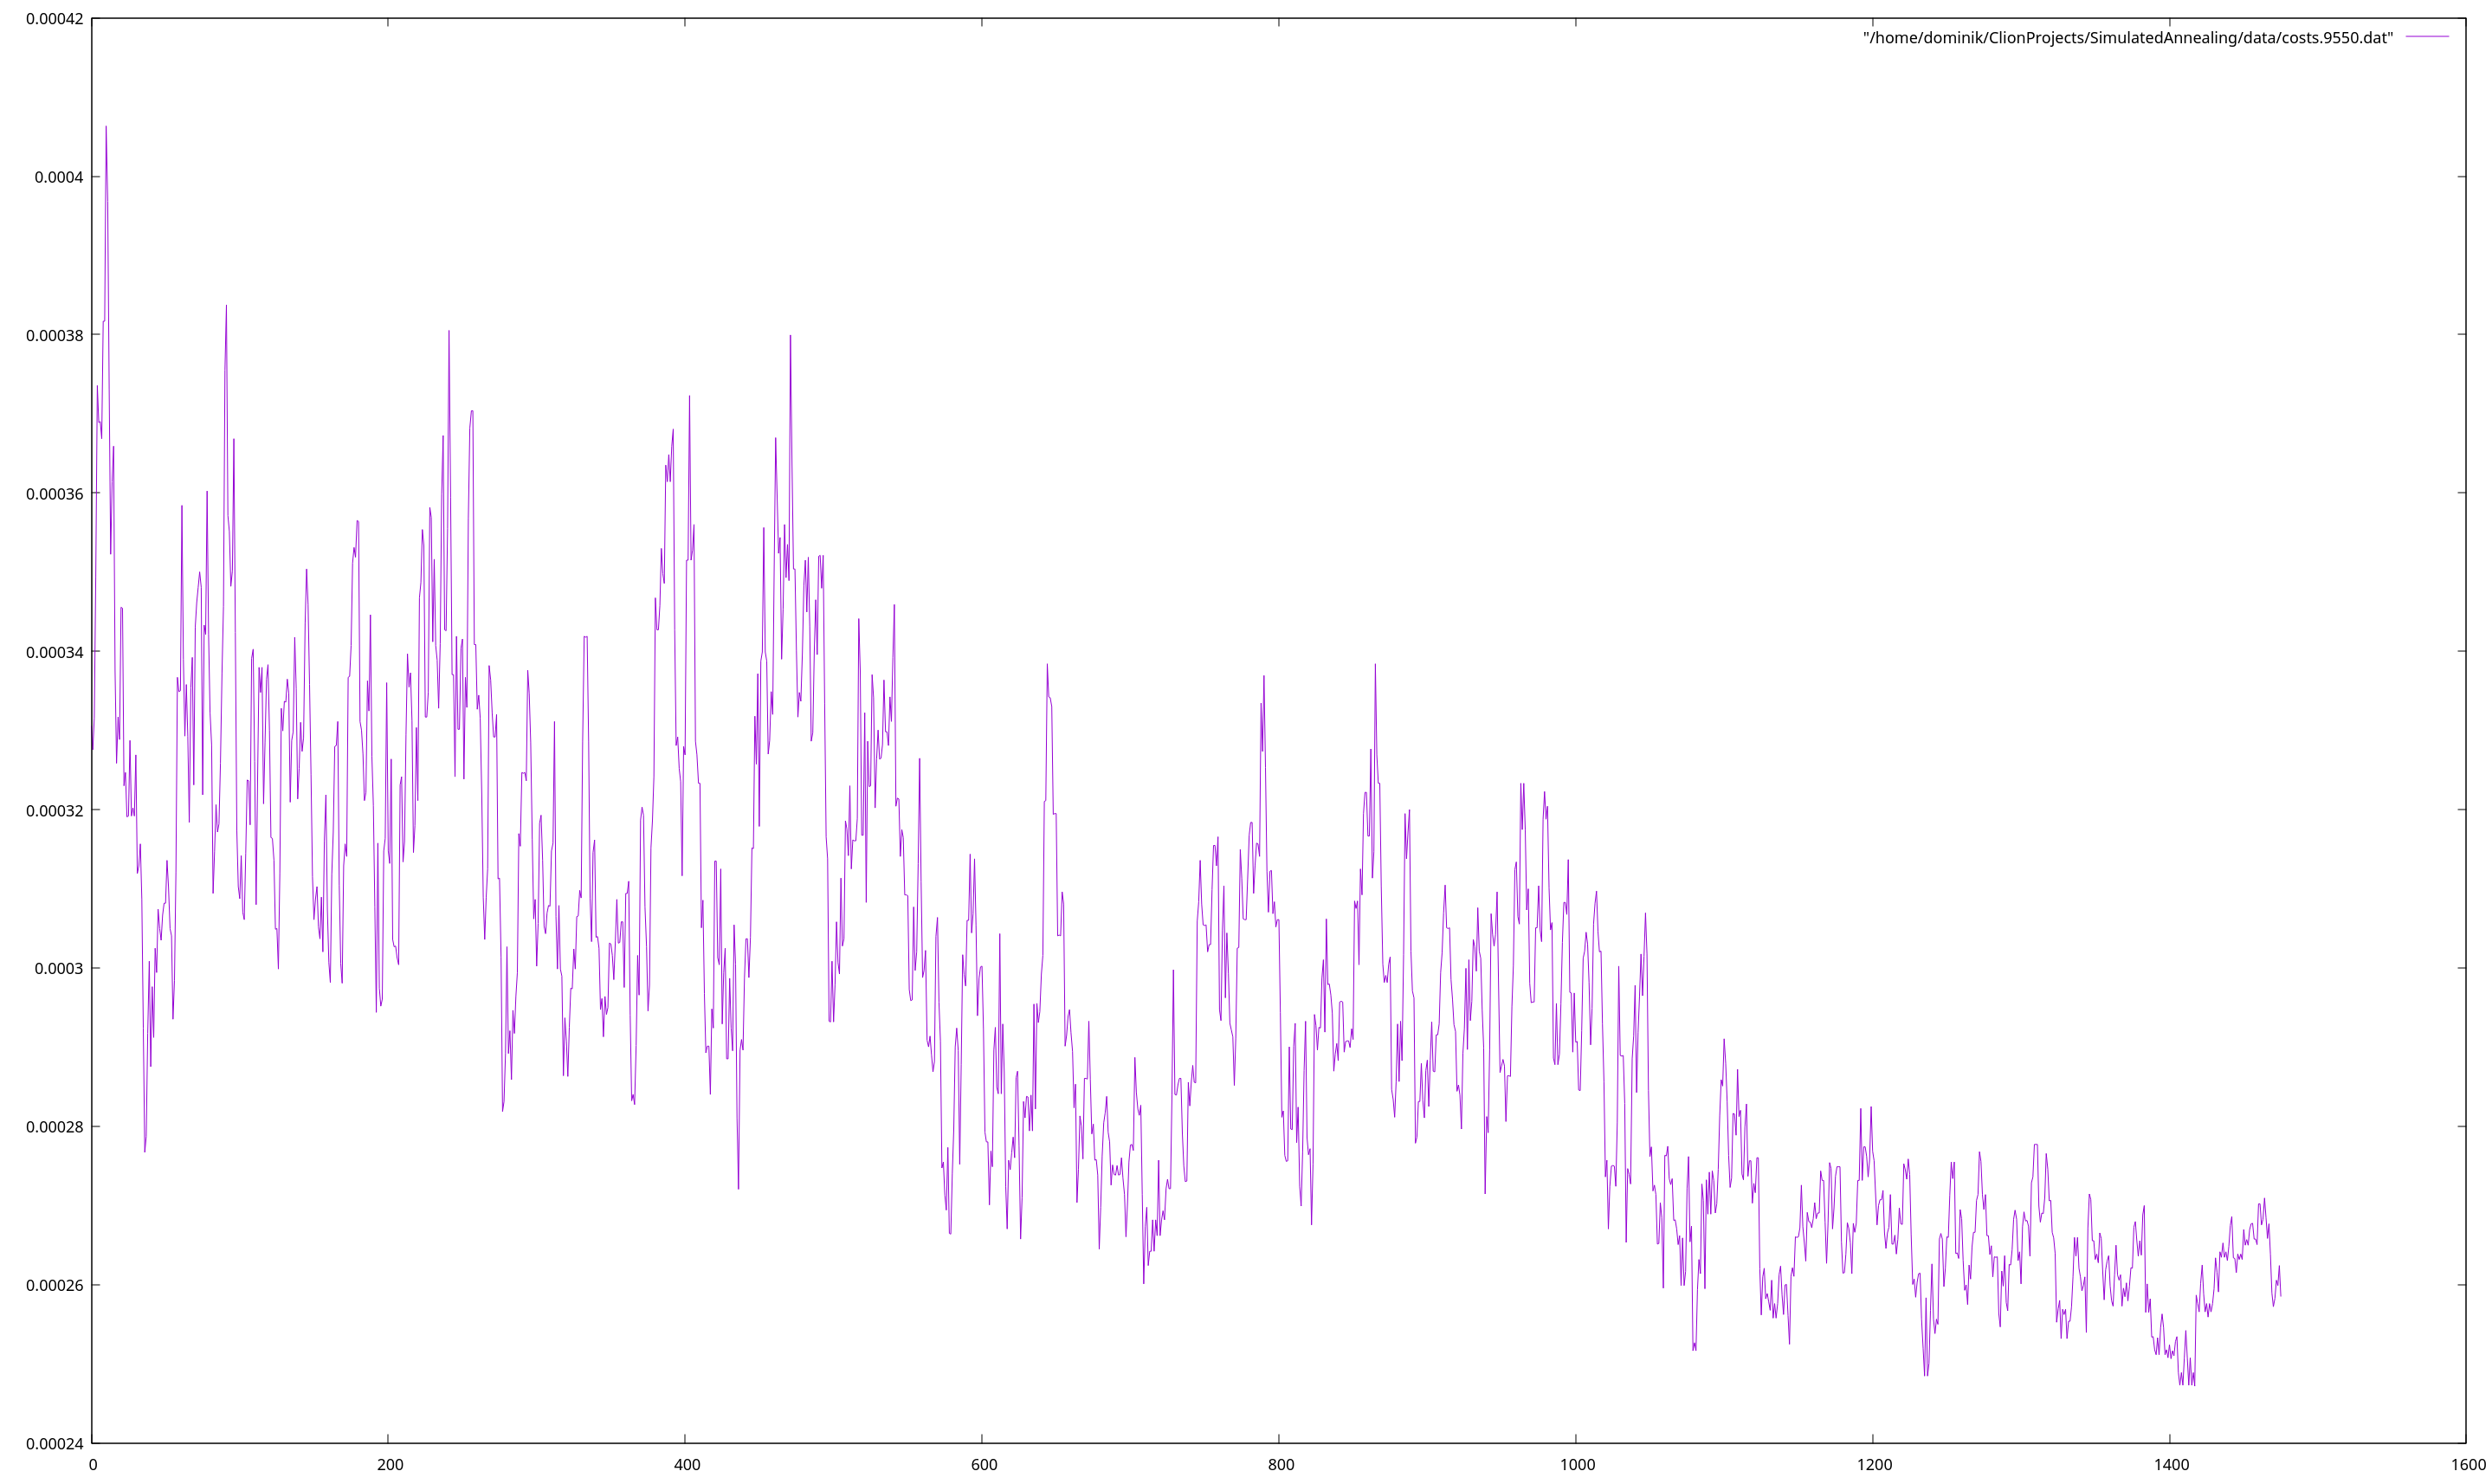
\includegraphics[width=\textwidth]{topCalcBottomCalc95}
\caption{Rychlost ochlazování 0,95 - rel. chyba 0.0054}
\label{topCalcBottomCalc95}
\end{figure}

\begin{figure}[H]
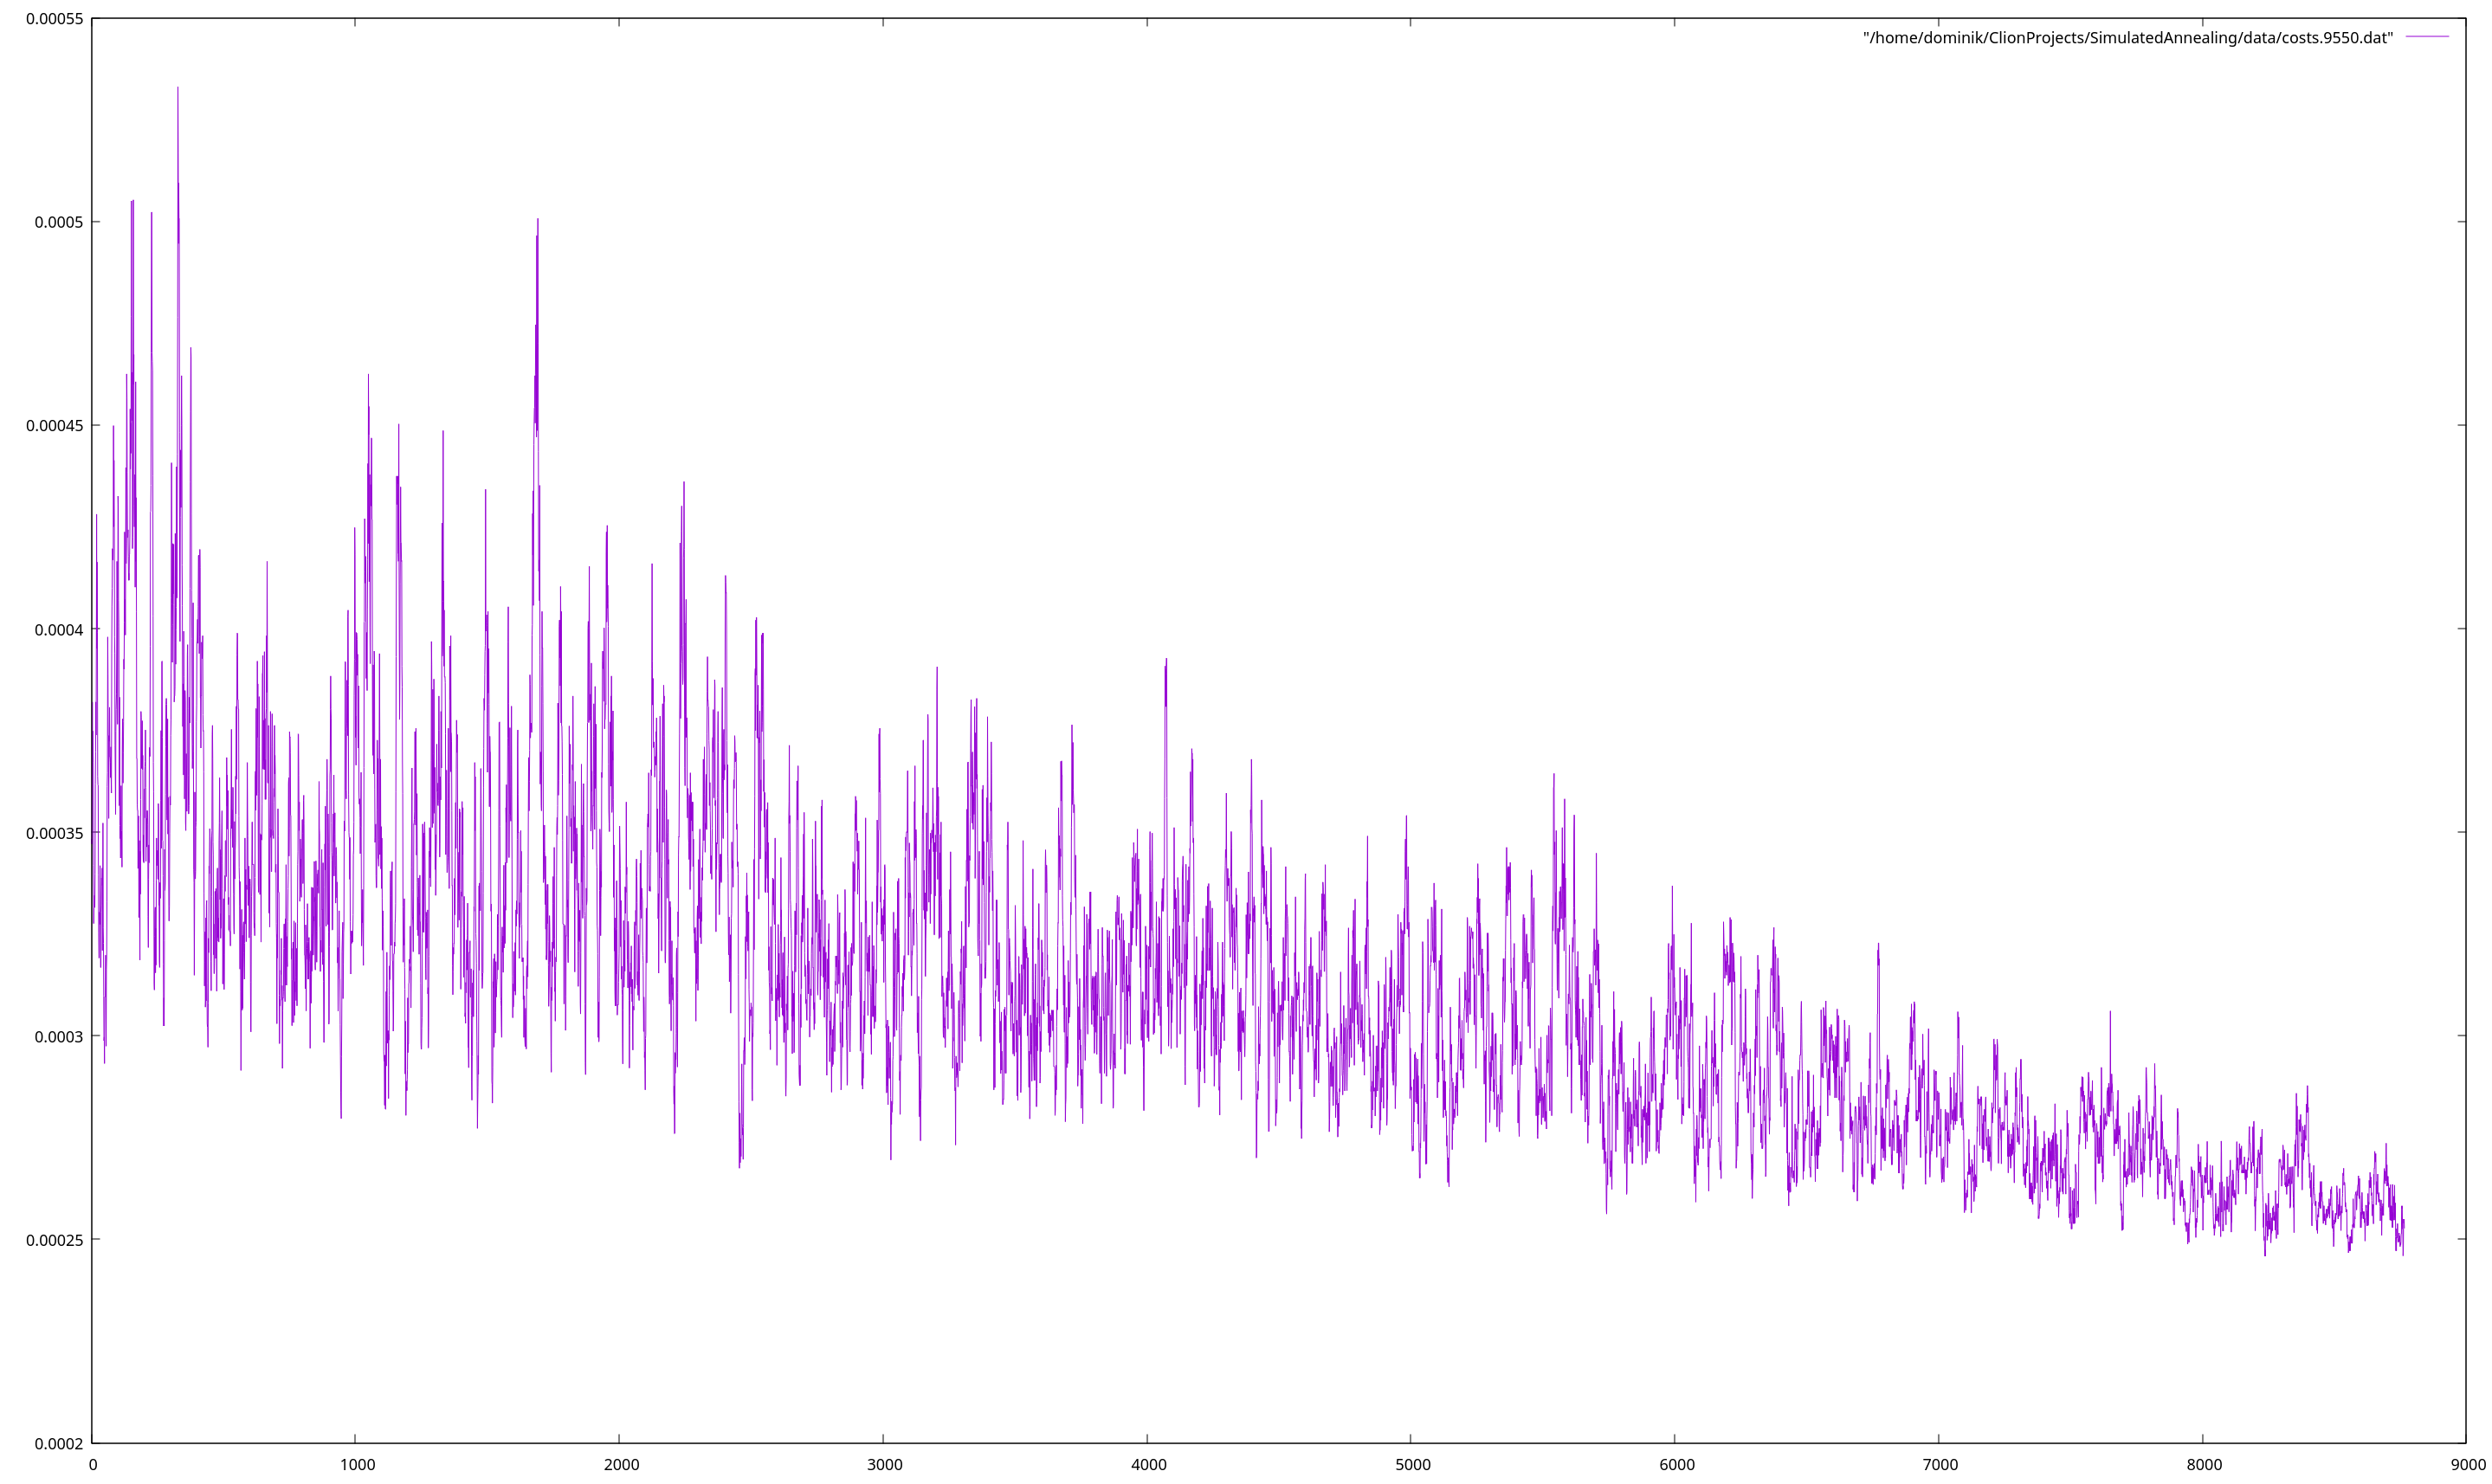
\includegraphics[width=\textwidth]{topCalcBottomCalc99}
\caption{Rychlost ochlazování 0,99 - rel. chyba 0.0}
\label{topCalcBottomCalc99}
\end{figure}


\subsection{Relativní chyby mnoha průběhů}
\label{sec_relerrs}

Jak je vidět, nejlepšího výsledku dosáhlo nejpomalejší ochlazování. To ale ještě není nutně průkazné, protože každý jeden průběh může být ovlivněn různými dalšími vlivy, jako je například náhodný výběr souseda. Proto jsem ještě spustil jeden test, kde jsem postupně snižoval rychlost ochlazování z 0.800 na 0.999. Pro každou z těchto 200 rychlostí jsem zaznamenal relativní chybu. Výsledek zobrazuje proložený graf \ref{relerrs}.

\begin{figure}[H]
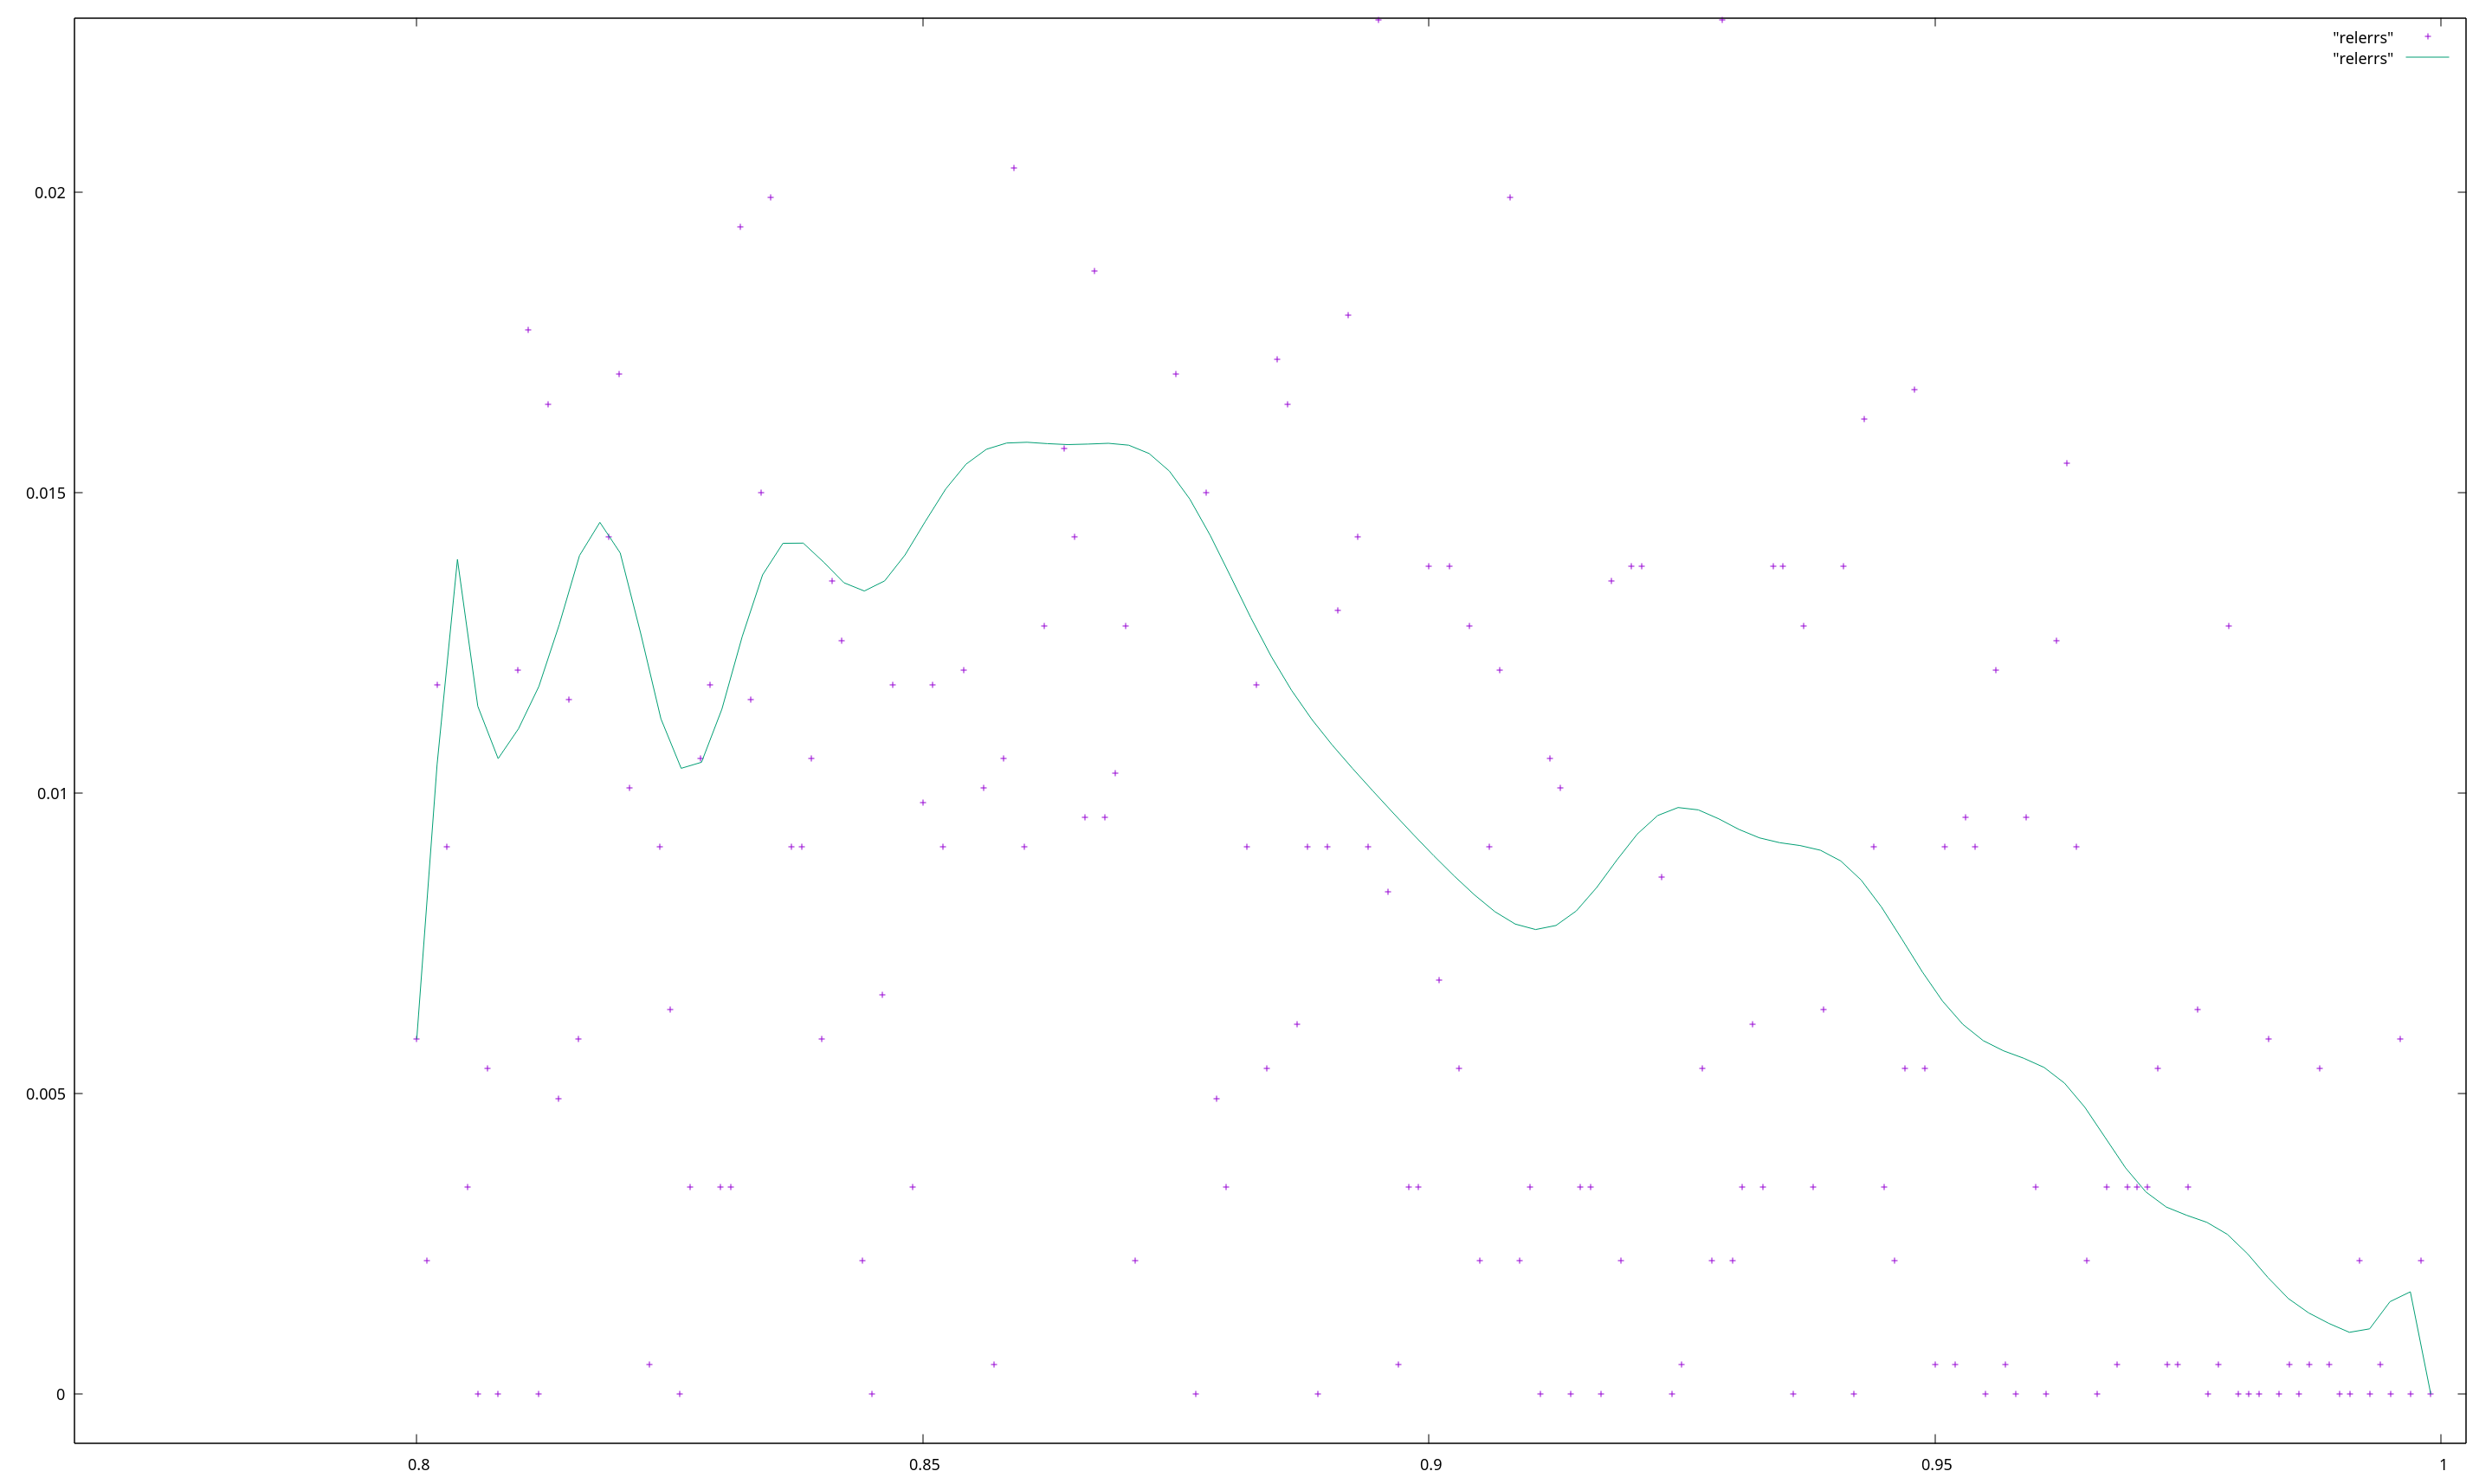
\includegraphics[width=\textwidth]{relerrs}
\caption{Vývoj relativní chyby v závislosti na rychlosti ochlazování}
\label{relerrs}
\end{figure}


\subsection{Čas výpočtu}

Dále bylo možné pozorovat, jak dlouho trvá výpočet, než dojde ke zmrznutí, v závislosti na zvolené rychlosti ochlazování. Stejný experiment jako v sekci \ref{sec_relerrs} vedl k nijak překvapivému zjištění, že čím pomalejší klesání teploty, tím déle výpočet trvá. Výsledek je vidět na proloženém grafu \ref{times}.

\begin{figure}[H]
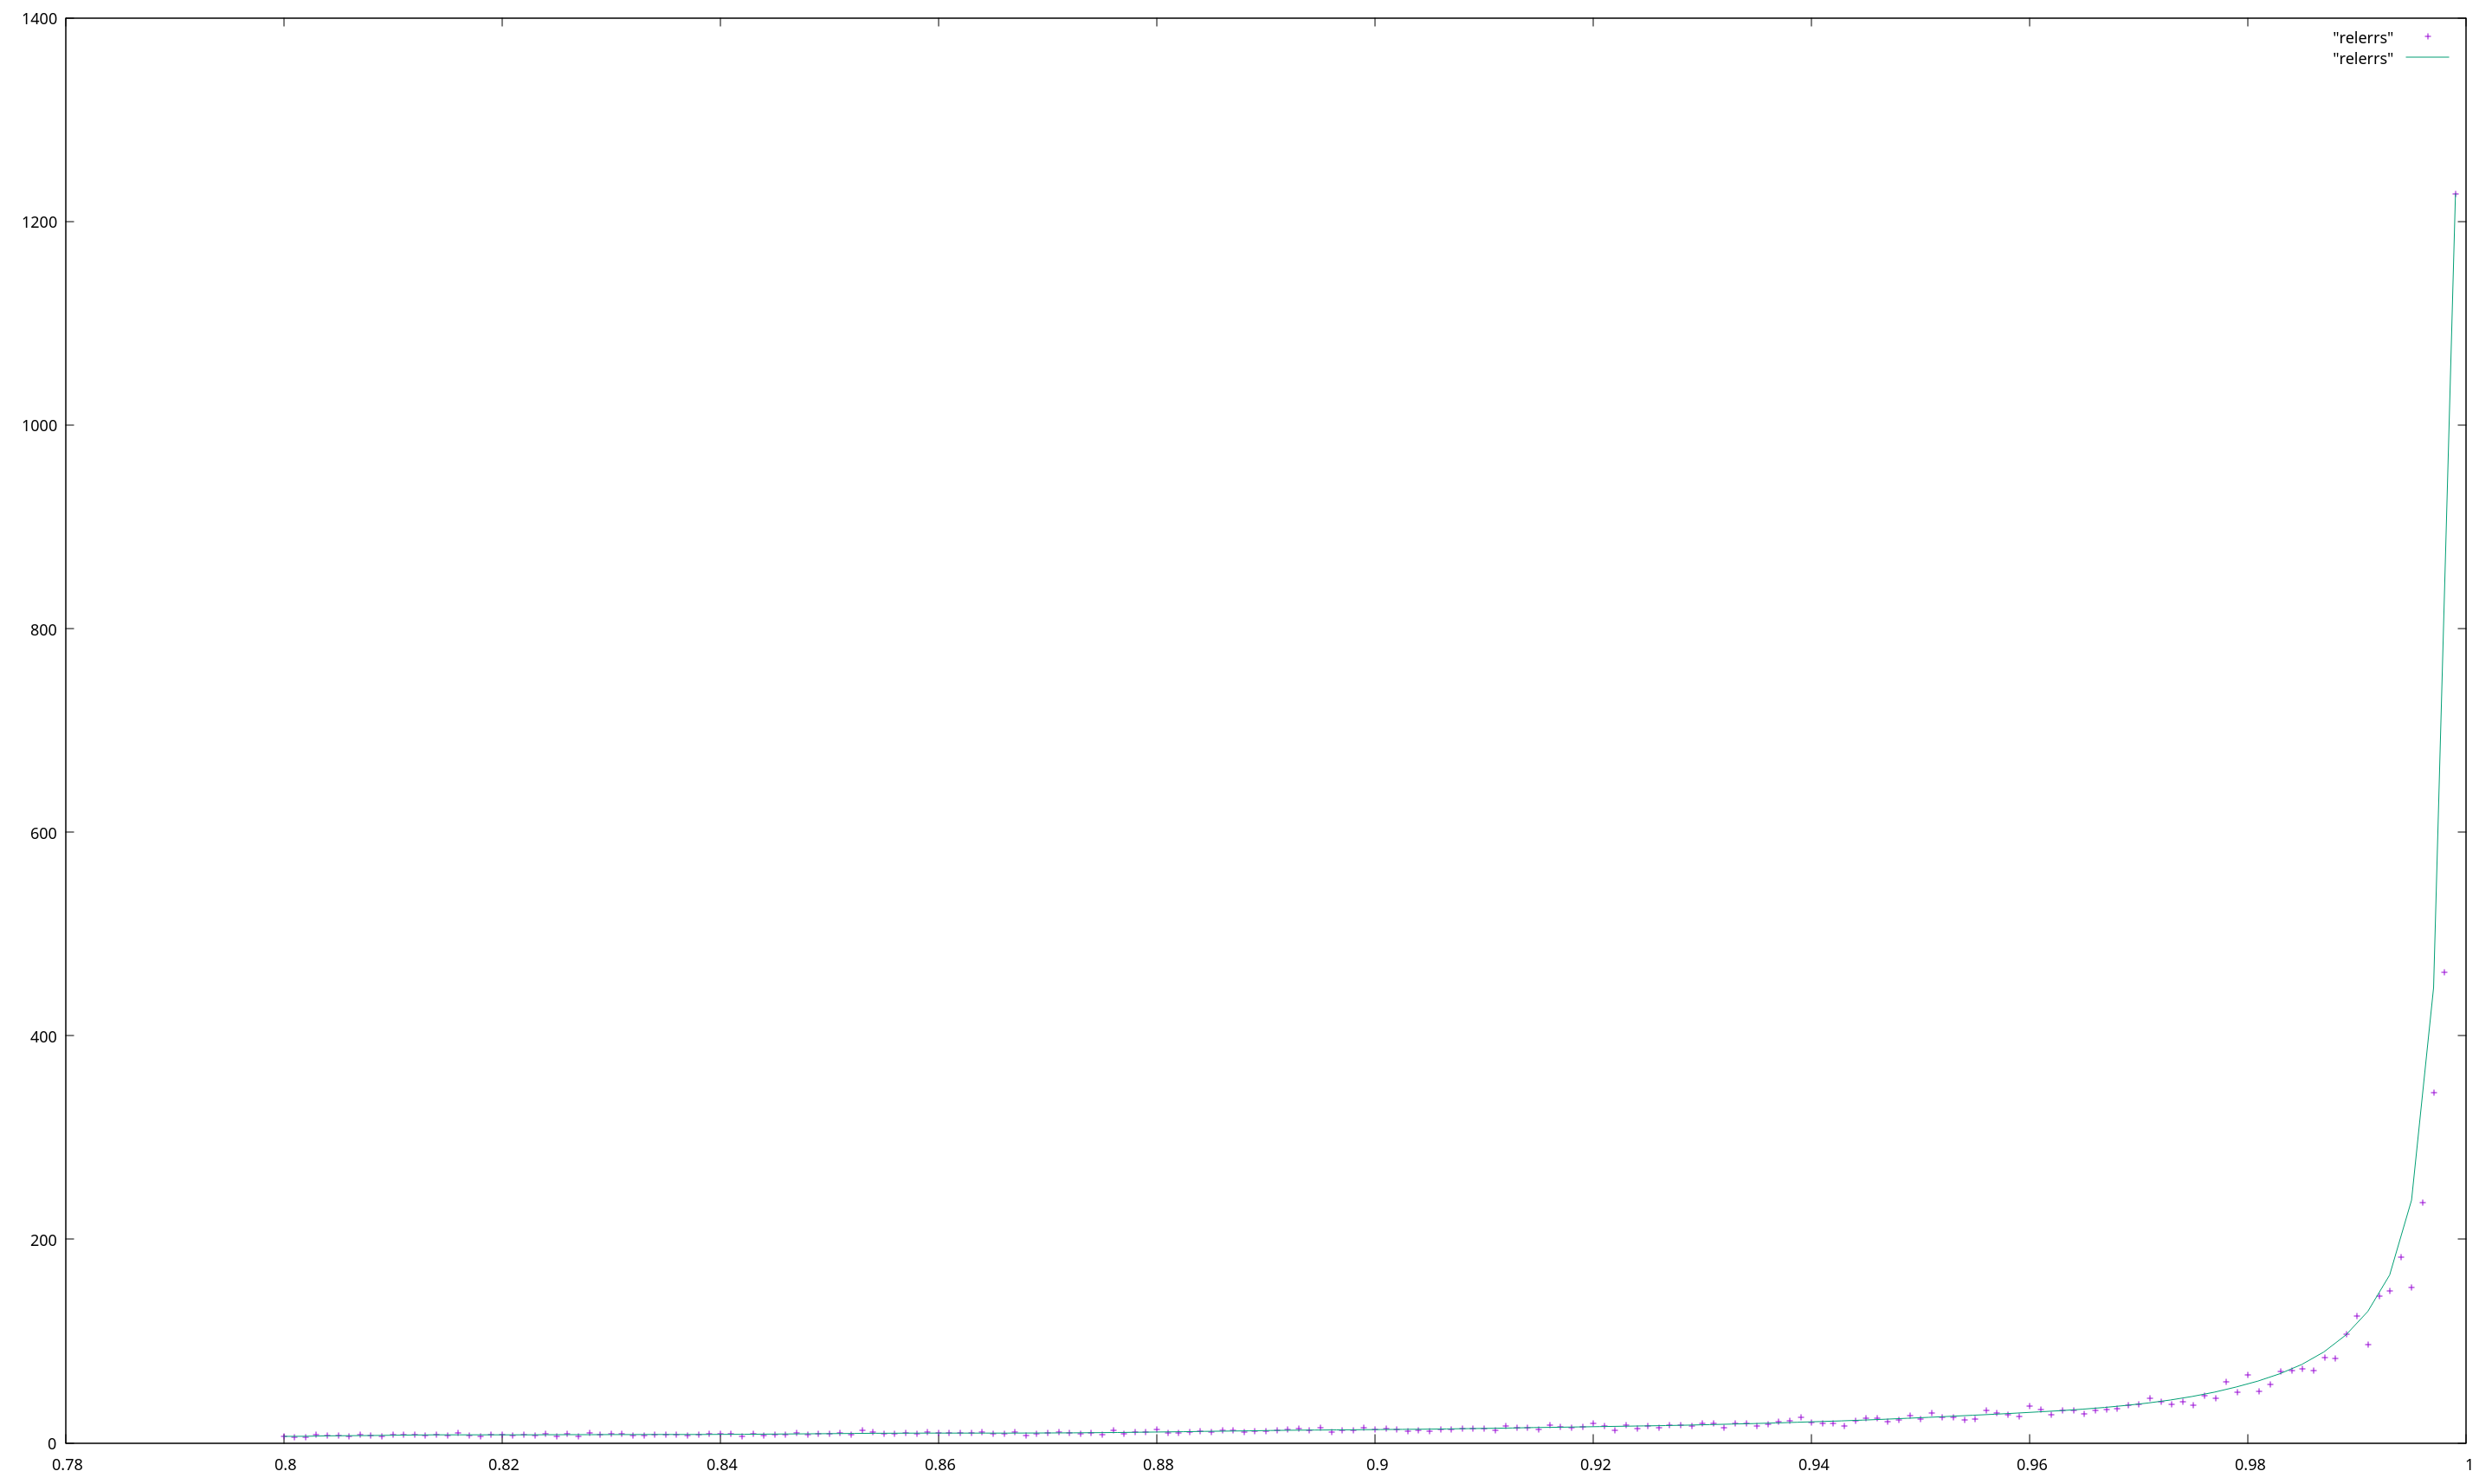
\includegraphics[width=\textwidth]{times}
\caption{Vývoj času výpočtu v závislosti na rychlosti ochlazování}
\label{times}
\end{figure}



\section{Závěr}

Je několik způsobů, jak implementovat metodu simulovaného ochlazování pro řešení problému batohu. V první řadě záleží na volbě, jak zacházet se skoky na stavy, které nejsou řešením, protože překračují kapacitu batohu. Zde jsem se rozhodl pro nejsnazší variantu, která by měla být i docela vyhovující a kterou, zdá se, používá poskytnutý applet, variantu ignorance. Dále záleží na volbě počáteční i koncové teploty. Zde jsem se rozhodl pro co nejobecnější přístup přes dynamický výpočet obojího.

V takto nastavených podmínkách jsem dospěl k závěru, že metoda simulovaného ochlazování řeší problém batohu velmi rychle a efektivně. I při velmi pomalém ochlazování s koeficientem přes 0.99 skončil výpočet do vteřiny a chyby se mnohdy pohybovaly v těsné blízkosti nuly, případně byly eliminovány zcela.

Dále se ukázalo, že čím pomalejší ochlazování, tím dosahuje metoda menší relativní chyby.



\end{document}